
\documentclass{article} % For LaTeX2e
\usepackage{iclr2026_conference,times}

% Optional math commands from https://github.com/goodfeli/dlbook_notation.
%%%%% NEW MATH DEFINITIONS %%%%%

\usepackage{amsmath,amsfonts,bm}

% Mark sections of captions for referring to divisions of figures
\newcommand{\figleft}{{\em (Left)}}
\newcommand{\figcenter}{{\em (Center)}}
\newcommand{\figright}{{\em (Right)}}
\newcommand{\figtop}{{\em (Top)}}
\newcommand{\figbottom}{{\em (Bottom)}}
\newcommand{\captiona}{{\em (a)}}
\newcommand{\captionb}{{\em (b)}}
\newcommand{\captionc}{{\em (c)}}
\newcommand{\captiond}{{\em (d)}}

% Highlight a newly defined term
\newcommand{\newterm}[1]{{\bf #1}}


% Figure reference, lower-case.
\def\figref#1{figure~\ref{#1}}
% Figure reference, capital. For start of sentence
\def\Figref#1{Figure~\ref{#1}}
\def\twofigref#1#2{figures \ref{#1} and \ref{#2}}
\def\quadfigref#1#2#3#4{figures \ref{#1}, \ref{#2}, \ref{#3} and \ref{#4}}
% Section reference, lower-case.
\def\secref#1{section~\ref{#1}}
% Section reference, capital.
\def\Secref#1{Section~\ref{#1}}
% Reference to two sections.
\def\twosecrefs#1#2{sections \ref{#1} and \ref{#2}}
% Reference to three sections.
\def\secrefs#1#2#3{sections \ref{#1}, \ref{#2} and \ref{#3}}
% Reference to an equation, lower-case.
\def\eqref#1{equation~\ref{#1}}
% Reference to an equation, upper case
\def\Eqref#1{Equation~\ref{#1}}
% A raw reference to an equation---avoid using if possible
\def\plaineqref#1{\ref{#1}}
% Reference to a chapter, lower-case.
\def\chapref#1{chapter~\ref{#1}}
% Reference to an equation, upper case.
\def\Chapref#1{Chapter~\ref{#1}}
% Reference to a range of chapters
\def\rangechapref#1#2{chapters\ref{#1}--\ref{#2}}
% Reference to an algorithm, lower-case.
\def\algref#1{algorithm~\ref{#1}}
% Reference to an algorithm, upper case.
\def\Algref#1{Algorithm~\ref{#1}}
\def\twoalgref#1#2{algorithms \ref{#1} and \ref{#2}}
\def\Twoalgref#1#2{Algorithms \ref{#1} and \ref{#2}}
% Reference to a part, lower case
\def\partref#1{part~\ref{#1}}
% Reference to a part, upper case
\def\Partref#1{Part~\ref{#1}}
\def\twopartref#1#2{parts \ref{#1} and \ref{#2}}

\def\ceil#1{\lceil #1 \rceil}
\def\floor#1{\lfloor #1 \rfloor}
\def\1{\bm{1}}
\newcommand{\train}{\mathcal{D}}
\newcommand{\valid}{\mathcal{D_{\mathrm{valid}}}}
\newcommand{\test}{\mathcal{D_{\mathrm{test}}}}

\def\eps{{\epsilon}}


% Random variables
\def\reta{{\textnormal{$\eta$}}}
\def\ra{{\textnormal{a}}}
\def\rb{{\textnormal{b}}}
\def\rc{{\textnormal{c}}}
\def\rd{{\textnormal{d}}}
\def\re{{\textnormal{e}}}
\def\rf{{\textnormal{f}}}
\def\rg{{\textnormal{g}}}
\def\rh{{\textnormal{h}}}
\def\ri{{\textnormal{i}}}
\def\rj{{\textnormal{j}}}
\def\rk{{\textnormal{k}}}
\def\rl{{\textnormal{l}}}
% rm is already a command, just don't name any random variables m
\def\rn{{\textnormal{n}}}
\def\ro{{\textnormal{o}}}
\def\rp{{\textnormal{p}}}
\def\rq{{\textnormal{q}}}
\def\rr{{\textnormal{r}}}
\def\rs{{\textnormal{s}}}
\def\rt{{\textnormal{t}}}
\def\ru{{\textnormal{u}}}
\def\rv{{\textnormal{v}}}
\def\rw{{\textnormal{w}}}
\def\rx{{\textnormal{x}}}
\def\ry{{\textnormal{y}}}
\def\rz{{\textnormal{z}}}

% Random vectors
\def\rvepsilon{{\mathbf{\epsilon}}}
\def\rvtheta{{\mathbf{\theta}}}
\def\rva{{\mathbf{a}}}
\def\rvb{{\mathbf{b}}}
\def\rvc{{\mathbf{c}}}
\def\rvd{{\mathbf{d}}}
\def\rve{{\mathbf{e}}}
\def\rvf{{\mathbf{f}}}
\def\rvg{{\mathbf{g}}}
\def\rvh{{\mathbf{h}}}
\def\rvu{{\mathbf{i}}}
\def\rvj{{\mathbf{j}}}
\def\rvk{{\mathbf{k}}}
\def\rvl{{\mathbf{l}}}
\def\rvm{{\mathbf{m}}}
\def\rvn{{\mathbf{n}}}
\def\rvo{{\mathbf{o}}}
\def\rvp{{\mathbf{p}}}
\def\rvq{{\mathbf{q}}}
\def\rvr{{\mathbf{r}}}
\def\rvs{{\mathbf{s}}}
\def\rvt{{\mathbf{t}}}
\def\rvu{{\mathbf{u}}}
\def\rvv{{\mathbf{v}}}
\def\rvw{{\mathbf{w}}}
\def\rvx{{\mathbf{x}}}
\def\rvy{{\mathbf{y}}}
\def\rvz{{\mathbf{z}}}

% Elements of random vectors
\def\erva{{\textnormal{a}}}
\def\ervb{{\textnormal{b}}}
\def\ervc{{\textnormal{c}}}
\def\ervd{{\textnormal{d}}}
\def\erve{{\textnormal{e}}}
\def\ervf{{\textnormal{f}}}
\def\ervg{{\textnormal{g}}}
\def\ervh{{\textnormal{h}}}
\def\ervi{{\textnormal{i}}}
\def\ervj{{\textnormal{j}}}
\def\ervk{{\textnormal{k}}}
\def\ervl{{\textnormal{l}}}
\def\ervm{{\textnormal{m}}}
\def\ervn{{\textnormal{n}}}
\def\ervo{{\textnormal{o}}}
\def\ervp{{\textnormal{p}}}
\def\ervq{{\textnormal{q}}}
\def\ervr{{\textnormal{r}}}
\def\ervs{{\textnormal{s}}}
\def\ervt{{\textnormal{t}}}
\def\ervu{{\textnormal{u}}}
\def\ervv{{\textnormal{v}}}
\def\ervw{{\textnormal{w}}}
\def\ervx{{\textnormal{x}}}
\def\ervy{{\textnormal{y}}}
\def\ervz{{\textnormal{z}}}

% Random matrices
\def\rmA{{\mathbf{A}}}
\def\rmB{{\mathbf{B}}}
\def\rmC{{\mathbf{C}}}
\def\rmD{{\mathbf{D}}}
\def\rmE{{\mathbf{E}}}
\def\rmF{{\mathbf{F}}}
\def\rmG{{\mathbf{G}}}
\def\rmH{{\mathbf{H}}}
\def\rmI{{\mathbf{I}}}
\def\rmJ{{\mathbf{J}}}
\def\rmK{{\mathbf{K}}}
\def\rmL{{\mathbf{L}}}
\def\rmM{{\mathbf{M}}}
\def\rmN{{\mathbf{N}}}
\def\rmO{{\mathbf{O}}}
\def\rmP{{\mathbf{P}}}
\def\rmQ{{\mathbf{Q}}}
\def\rmR{{\mathbf{R}}}
\def\rmS{{\mathbf{S}}}
\def\rmT{{\mathbf{T}}}
\def\rmU{{\mathbf{U}}}
\def\rmV{{\mathbf{V}}}
\def\rmW{{\mathbf{W}}}
\def\rmX{{\mathbf{X}}}
\def\rmY{{\mathbf{Y}}}
\def\rmZ{{\mathbf{Z}}}

% Elements of random matrices
\def\ermA{{\textnormal{A}}}
\def\ermB{{\textnormal{B}}}
\def\ermC{{\textnormal{C}}}
\def\ermD{{\textnormal{D}}}
\def\ermE{{\textnormal{E}}}
\def\ermF{{\textnormal{F}}}
\def\ermG{{\textnormal{G}}}
\def\ermH{{\textnormal{H}}}
\def\ermI{{\textnormal{I}}}
\def\ermJ{{\textnormal{J}}}
\def\ermK{{\textnormal{K}}}
\def\ermL{{\textnormal{L}}}
\def\ermM{{\textnormal{M}}}
\def\ermN{{\textnormal{N}}}
\def\ermO{{\textnormal{O}}}
\def\ermP{{\textnormal{P}}}
\def\ermQ{{\textnormal{Q}}}
\def\ermR{{\textnormal{R}}}
\def\ermS{{\textnormal{S}}}
\def\ermT{{\textnormal{T}}}
\def\ermU{{\textnormal{U}}}
\def\ermV{{\textnormal{V}}}
\def\ermW{{\textnormal{W}}}
\def\ermX{{\textnormal{X}}}
\def\ermY{{\textnormal{Y}}}
\def\ermZ{{\textnormal{Z}}}

% Vectors
\def\vzero{{\bm{0}}}
\def\vone{{\bm{1}}}
\def\vmu{{\bm{\mu}}}
\def\vtheta{{\bm{\theta}}}
\def\va{{\bm{a}}}
\def\vb{{\bm{b}}}
\def\vc{{\bm{c}}}
\def\vd{{\bm{d}}}
\def\ve{{\bm{e}}}
\def\vf{{\bm{f}}}
\def\vg{{\bm{g}}}
\def\vh{{\bm{h}}}
\def\vi{{\bm{i}}}
\def\vj{{\bm{j}}}
\def\vk{{\bm{k}}}
\def\vl{{\bm{l}}}
\def\vm{{\bm{m}}}
\def\vn{{\bm{n}}}
\def\vo{{\bm{o}}}
\def\vp{{\bm{p}}}
\def\vq{{\bm{q}}}
\def\vr{{\bm{r}}}
\def\vs{{\bm{s}}}
\def\vt{{\bm{t}}}
\def\vu{{\bm{u}}}
\def\vv{{\bm{v}}}
\def\vw{{\bm{w}}}
\def\vx{{\bm{x}}}
\def\vy{{\bm{y}}}
\def\vz{{\bm{z}}}

% Elements of vectors
\def\evalpha{{\alpha}}
\def\evbeta{{\beta}}
\def\evepsilon{{\epsilon}}
\def\evlambda{{\lambda}}
\def\evomega{{\omega}}
\def\evmu{{\mu}}
\def\evpsi{{\psi}}
\def\evsigma{{\sigma}}
\def\evtheta{{\theta}}
\def\eva{{a}}
\def\evb{{b}}
\def\evc{{c}}
\def\evd{{d}}
\def\eve{{e}}
\def\evf{{f}}
\def\evg{{g}}
\def\evh{{h}}
\def\evi{{i}}
\def\evj{{j}}
\def\evk{{k}}
\def\evl{{l}}
\def\evm{{m}}
\def\evn{{n}}
\def\evo{{o}}
\def\evp{{p}}
\def\evq{{q}}
\def\evr{{r}}
\def\evs{{s}}
\def\evt{{t}}
\def\evu{{u}}
\def\evv{{v}}
\def\evw{{w}}
\def\evx{{x}}
\def\evy{{y}}
\def\evz{{z}}

% Matrix
\def\mA{{\bm{A}}}
\def\mB{{\bm{B}}}
\def\mC{{\bm{C}}}
\def\mD{{\bm{D}}}
\def\mE{{\bm{E}}}
\def\mF{{\bm{F}}}
\def\mG{{\bm{G}}}
\def\mH{{\bm{H}}}
\def\mI{{\bm{I}}}
\def\mJ{{\bm{J}}}
\def\mK{{\bm{K}}}
\def\mL{{\bm{L}}}
\def\mM{{\bm{M}}}
\def\mN{{\bm{N}}}
\def\mO{{\bm{O}}}
\def\mP{{\bm{P}}}
\def\mQ{{\bm{Q}}}
\def\mR{{\bm{R}}}
\def\mS{{\bm{S}}}
\def\mT{{\bm{T}}}
\def\mU{{\bm{U}}}
\def\mV{{\bm{V}}}
\def\mW{{\bm{W}}}
\def\mX{{\bm{X}}}
\def\mY{{\bm{Y}}}
\def\mZ{{\bm{Z}}}
\def\mBeta{{\bm{\beta}}}
\def\mPhi{{\bm{\Phi}}}
\def\mLambda{{\bm{\Lambda}}}
\def\mSigma{{\bm{\Sigma}}}

% Tensor
\DeclareMathAlphabet{\mathsfit}{\encodingdefault}{\sfdefault}{m}{sl}
\SetMathAlphabet{\mathsfit}{bold}{\encodingdefault}{\sfdefault}{bx}{n}
\newcommand{\tens}[1]{\bm{\mathsfit{#1}}}
\def\tA{{\tens{A}}}
\def\tB{{\tens{B}}}
\def\tC{{\tens{C}}}
\def\tD{{\tens{D}}}
\def\tE{{\tens{E}}}
\def\tF{{\tens{F}}}
\def\tG{{\tens{G}}}
\def\tH{{\tens{H}}}
\def\tI{{\tens{I}}}
\def\tJ{{\tens{J}}}
\def\tK{{\tens{K}}}
\def\tL{{\tens{L}}}
\def\tM{{\tens{M}}}
\def\tN{{\tens{N}}}
\def\tO{{\tens{O}}}
\def\tP{{\tens{P}}}
\def\tQ{{\tens{Q}}}
\def\tR{{\tens{R}}}
\def\tS{{\tens{S}}}
\def\tT{{\tens{T}}}
\def\tU{{\tens{U}}}
\def\tV{{\tens{V}}}
\def\tW{{\tens{W}}}
\def\tX{{\tens{X}}}
\def\tY{{\tens{Y}}}
\def\tZ{{\tens{Z}}}


% Graph
\def\gA{{\mathcal{A}}}
\def\gB{{\mathcal{B}}}
\def\gC{{\mathcal{C}}}
\def\gD{{\mathcal{D}}}
\def\gE{{\mathcal{E}}}
\def\gF{{\mathcal{F}}}
\def\gG{{\mathcal{G}}}
\def\gH{{\mathcal{H}}}
\def\gI{{\mathcal{I}}}
\def\gJ{{\mathcal{J}}}
\def\gK{{\mathcal{K}}}
\def\gL{{\mathcal{L}}}
\def\gM{{\mathcal{M}}}
\def\gN{{\mathcal{N}}}
\def\gO{{\mathcal{O}}}
\def\gP{{\mathcal{P}}}
\def\gQ{{\mathcal{Q}}}
\def\gR{{\mathcal{R}}}
\def\gS{{\mathcal{S}}}
\def\gT{{\mathcal{T}}}
\def\gU{{\mathcal{U}}}
\def\gV{{\mathcal{V}}}
\def\gW{{\mathcal{W}}}
\def\gX{{\mathcal{X}}}
\def\gY{{\mathcal{Y}}}
\def\gZ{{\mathcal{Z}}}

% Sets
\def\sA{{\mathbb{A}}}
\def\sB{{\mathbb{B}}}
\def\sC{{\mathbb{C}}}
\def\sD{{\mathbb{D}}}
% Don't use a set called E, because this would be the same as our symbol
% for expectation.
\def\sF{{\mathbb{F}}}
\def\sG{{\mathbb{G}}}
\def\sH{{\mathbb{H}}}
\def\sI{{\mathbb{I}}}
\def\sJ{{\mathbb{J}}}
\def\sK{{\mathbb{K}}}
\def\sL{{\mathbb{L}}}
\def\sM{{\mathbb{M}}}
\def\sN{{\mathbb{N}}}
\def\sO{{\mathbb{O}}}
\def\sP{{\mathbb{P}}}
\def\sQ{{\mathbb{Q}}}
\def\sR{{\mathbb{R}}}
\def\sS{{\mathbb{S}}}
\def\sT{{\mathbb{T}}}
\def\sU{{\mathbb{U}}}
\def\sV{{\mathbb{V}}}
\def\sW{{\mathbb{W}}}
\def\sX{{\mathbb{X}}}
\def\sY{{\mathbb{Y}}}
\def\sZ{{\mathbb{Z}}}

% Entries of a matrix
\def\emLambda{{\Lambda}}
\def\emA{{A}}
\def\emB{{B}}
\def\emC{{C}}
\def\emD{{D}}
\def\emE{{E}}
\def\emF{{F}}
\def\emG{{G}}
\def\emH{{H}}
\def\emI{{I}}
\def\emJ{{J}}
\def\emK{{K}}
\def\emL{{L}}
\def\emM{{M}}
\def\emN{{N}}
\def\emO{{O}}
\def\emP{{P}}
\def\emQ{{Q}}
\def\emR{{R}}
\def\emS{{S}}
\def\emT{{T}}
\def\emU{{U}}
\def\emV{{V}}
\def\emW{{W}}
\def\emX{{X}}
\def\emY{{Y}}
\def\emZ{{Z}}
\def\emSigma{{\Sigma}}

% entries of a tensor
% Same font as tensor, without \bm wrapper
\newcommand{\etens}[1]{\mathsfit{#1}}
\def\etLambda{{\etens{\Lambda}}}
\def\etA{{\etens{A}}}
\def\etB{{\etens{B}}}
\def\etC{{\etens{C}}}
\def\etD{{\etens{D}}}
\def\etE{{\etens{E}}}
\def\etF{{\etens{F}}}
\def\etG{{\etens{G}}}
\def\etH{{\etens{H}}}
\def\etI{{\etens{I}}}
\def\etJ{{\etens{J}}}
\def\etK{{\etens{K}}}
\def\etL{{\etens{L}}}
\def\etM{{\etens{M}}}
\def\etN{{\etens{N}}}
\def\etO{{\etens{O}}}
\def\etP{{\etens{P}}}
\def\etQ{{\etens{Q}}}
\def\etR{{\etens{R}}}
\def\etS{{\etens{S}}}
\def\etT{{\etens{T}}}
\def\etU{{\etens{U}}}
\def\etV{{\etens{V}}}
\def\etW{{\etens{W}}}
\def\etX{{\etens{X}}}
\def\etY{{\etens{Y}}}
\def\etZ{{\etens{Z}}}

% The true underlying data generating distribution
\newcommand{\pdata}{p_{\rm{data}}}
% The empirical distribution defined by the training set
\newcommand{\ptrain}{\hat{p}_{\rm{data}}}
\newcommand{\Ptrain}{\hat{P}_{\rm{data}}}
% The model distribution
\newcommand{\pmodel}{p_{\rm{model}}}
\newcommand{\Pmodel}{P_{\rm{model}}}
\newcommand{\ptildemodel}{\tilde{p}_{\rm{model}}}
% Stochastic autoencoder distributions
\newcommand{\pencode}{p_{\rm{encoder}}}
\newcommand{\pdecode}{p_{\rm{decoder}}}
\newcommand{\precons}{p_{\rm{reconstruct}}}

\newcommand{\laplace}{\mathrm{Laplace}} % Laplace distribution

\newcommand{\E}{\mathbb{E}}
\newcommand{\Ls}{\mathcal{L}}
\newcommand{\R}{\mathbb{R}}
\newcommand{\emp}{\tilde{p}}
\newcommand{\lr}{\alpha}
\newcommand{\reg}{\lambda}
\newcommand{\rect}{\mathrm{rectifier}}
\newcommand{\softmax}{\mathrm{softmax}}
\newcommand{\sigmoid}{\sigma}
\newcommand{\softplus}{\zeta}
\newcommand{\KL}{D_{\mathrm{KL}}}
\newcommand{\Var}{\mathrm{Var}}
\newcommand{\standarderror}{\mathrm{SE}}
\newcommand{\Cov}{\mathrm{Cov}}
% Wolfram Mathworld says $L^2$ is for function spaces and $\ell^2$ is for vectors
% But then they seem to use $L^2$ for vectors throughout the site, and so does
% wikipedia.
\newcommand{\normlzero}{L^0}
\newcommand{\normlone}{L^1}
\newcommand{\normltwo}{L^2}
\newcommand{\normlp}{L^p}
\newcommand{\normmax}{L^\infty}

\newcommand{\parents}{Pa} % See usage in notation.tex. Chosen to match Daphne's book.

\DeclareMathOperator*{\argmax}{arg\,max}
\DeclareMathOperator*{\argmin}{arg\,min}

\DeclareMathOperator{\sign}{sign}
\DeclareMathOperator{\Tr}{Tr}
\let\ab\allowbreak


\usepackage{hyperref}
\usepackage{url}
\usepackage{rotating}
% zhangmin
\usepackage{booktabs}       % professional-quality tables
\usepackage{tabularx}
\usepackage{graphicx} % Required for \resizebox
\definecolor{darkgrey}{rgb}{0.53,0.53,0.53}
\definecolor{mygrey}{rgb}{0.9,0.9,0.9}
\definecolor{blue1}{RGB}{166, 206, 227}
\definecolor{blue2}{RGB}{28, 118, 179}
\definecolor{myorange}{RGB}{192,97,21}
\usepackage[most]{tcolorbox}
\usepackage{CJKutf8}
\newcommand{\cc}[1]{\begin{CJK*}{UTF8}{gbsn}#1\end{CJK*}}
\usepackage{hyperref}
\usepackage{multirow}

\title{OmniEduBench: A Comprehensive Chinese Benchmark for Evaluating Large Language Models in Education}


% Authors must not appear in the submitted version. They should be hidden
% as long as the \iclrfinalcopy macro remains commented out below.
% Non-anonymous submissions will be rejected without review.

\author{
Min Zhang$^{1}$\thanks{Project leader. Min Zhang (mzhang@cs.ecnu.edu.cn) } \quad 
Hao Chen$^{1}$ \quad 
Wenqi Zhang$^{2}$ \quad 
Didi Zhu$^{3}$ \quad 
Xin Lin$^{1}$ \quad 
Bo Jiang$^{1}$\thanks{Corresponding authors. Bo Jiang (bjiang@deit.ecnu.edu.cn) and Aimin Zhou (amzhou@cs.ecnu.edu.cn)} \\[0.3em] 
\ \textbf{Aimin Zhou}$^{1\dagger}$ \quad 
\textbf{Fei Wu}$^{2}$ \quad 
\textbf{Kun Kuang}$^{2}$ \\[0.3em]
$^{1}$East China Normal University \quad 
$^{2}$Zhejiang University \quad 
$^{3}$Imperial College London \\[0.3em]
{\tt\small mzhang@cs.ecnu.edu.cn} \quad
{\tt\small bjiang@deit.ecnu.edu.cn} \quad
{\tt\small amzhou@cs.ecnu.edu.cn} \\[0.5em]
\quad \quad \quad \quad \quad \quad \quad \quad \quad \quad \url{https://omniedubench.github.io/}
}


% The \author macro works with any number of authors. There are two commands
% used to separate the names and addresses of multiple authors: \And and \AND.
%
% Using \And between authors leaves it to \LaTeX{} to determine where to break
% the lines. Using \AND forces a linebreak at that point. So, if \LaTeX{}
% puts 3 of 4 authors names on the first line, and the last on the second
% line, try using \AND instead of \And before the third author name.

\newcommand{\fix}{\marginpar{FIX}}
\newcommand{\new}{\marginpar{NEW}}

%\iclrfinalcopy % Uncomment for camera-ready version, but NOT for submission.

% \iclrfinalcopy

\begin{document}


\maketitle

\begin{abstract}
    With the rapid development of large language models (LLMs), various LLM-based works have been widely applied in educational fields. However, most existing LLMs and their benchmarks focus primarily on \textit{the knowledge dimension, largely neglecting the evaluation of cultivation capabilities} that are essential for real-world educational scenarios. Additionally, current benchmarks are often \textit{limited to a single subject or question type, lacking sufficient diversity}. This issue is particularly prominent within the Chinese context. To address this gap, we introduce \textbf{OmniEduBench, a comprehensive Chinese educational benchmark}. OmniEduBench consists of 24.602K high-quality question-answer pairs. The data is meticulously divided into two core dimensions: \textbf{the knowledge dimension and the cultivation dimension}, which contain 18.121K and 6.481K entries, respectively. Each dimension is further subdivided into 6 fine-grained categories, covering a total of 61 different subjects (41 in the knowledge and 20 in the cultivation). Furthermore, the dataset features a rich variety of question formats, including 11 common exam question types, providing a solid foundation for comprehensively evaluating LLMs' capabilities in education. Extensive experiments on 11 mainstream open-source and closed-source LLMs reveal a clear performance gap. In the knowledge dimension, only Gemini-2.5 Pro surpassed 60\% accuracy, while in the cultivation dimension, the best-performing model, QWQ, still trailed human intelligence by nearly 30\%. These results highlight the substantial room for improvement and underscore the challenges of applying LLMs in education.
\end{abstract}

\section{Introduction}

With the rapid emergence of large language models (LLMs), evaluation benchmarks have become increasingly critical, shifting the focus of assessment toward broader and complex skills. To address the demands of this complex paradigm, a variety of benchmarks have been proposed to evaluate the diverse capabilities of LLMs. These benchmarks cover a wide spectrum of areas, including knowledge and language understanding (\textit{e.g.}, MMLU~\citep{hendrycks2021measuring}, ARC~\citep{allenai:arc}), reasoning (\textit{e.g.}, GSM8K~\citep{cobbe2021gsm8k}, AIME~\citep{patel2024aime}), multi-turn open-ended dialogue (\textit{e.g.}, MT-bench~\citep{bai2024mt}), and coding (\textit{e.g.}, MBPP~\citep{austin2021program}). Serving as indispensable tools for advancing LLM development, these benchmarks have been widely adopted in recent influential works~\citep{hurst2024gpt-4o,liu2024deepseek-v2,seed2025seed-oss,comanici2025gemini,taylor2022galactica,touvron2023llama,openai2023gpt4,hoffmann2022training}.

In recent years, a series of powerful Chinese LLMs emerged, such as the Qwen~\citep{qwen2.5,yang2025qwen3}, DeepSeek~\citep{liu2024deepseek-v2,guo2025deepseek,liu2024deepseek-v3}, achieving performance levels comparable to overseas LLMs. With the growing application of LLMs in education, researchers have also begun to propose Chinese education benchmarks, which can be broadly categorized into two types: \textcolor{blue2}{(1) datasets translated from other languages} and \textcolor{myorange}{(2) datasets natively constructed from Chinese education corpora}. Specifically, \textcolor{blue2}{(1) Datasets translated from other languages} refer to benchmarks constructed by directly translating existing benchmarks from other languages into Chinese. A representative work is CLUE~\citep{xu-etal-2020-clue}, which was translated from the English GLUE~\citep{wangglue}.
However, a simple translation approach is insufficient for a rigorous evaluation of LLMs in Chinese. These datasets often fail to reflect the unique linguistic and cultural challenges of the Chinese education and inherently carry biases from their original environment, thus limiting their ability to assess LLMs’ understanding of local education knowledge and teacher-student needs.

\textcolor{myorange}{(2) Datasets natively constructed from Chinese educational corpora} refer to benchmarks directly collected from Chinese educational text resources, such as C-Eval~\citep{huang2023ceval}, Edubench~\citep{xu2025edubench}, Scieval~\citep{sun2024scieval}, AGIEval~\citep{zhong2023agieval}, and SuperCLUE~\citep{xu2023superclue}. However, most existing education benchmarks are often limited to a single subject or question type, lacking sufficient diversity. Additionally, these datasets typically focus on the knowledge dimension, overlooking the unique cultivation aspects that are essential in real-world education. 

% This naturally raises a pivotal question:

% \begin{tcolorbox}[notitle, rounded corners, colframe=myorange, colback=white, boxrule=2pt, boxsep=0pt, left=0.15cm, right=0.17cm, enhanced, shadow={2.5pt}{-2.5pt}{0pt}{opacity=5,mygrey},toprule=2pt, before skip=0.65em, after skip=0.75em]
% \emph{
%   {
%     \centering 
%   {
%     \fontsize{8pt}{13.2pt}\selectfont 
%     How can we develop a natively Chinese evaluation benchmark that captures the unique linguistic and cultural knowledge of Chinese, incorporates diverse question types, and assesses large language models (LLMs) not only on the knowledge dimension but also on the distinctive Cultivation competencies required in realistic educational settings?
%   }
%   \\
%   }
%   }
% \end{tcolorbox}

We present OmniEduBench, a comprehensive Chinese education benchmark designed to thoroughly evaluate LLMs in terms of both knowledge understanding and skill cultivation in educational scenarios. OmniEduBench encompasses knowledge and cultivation dimension and comprises a total of 24.602K high-quality question–answer pairs, covering 11 common exam question types (\textit{e.g.}, multiple choice (\cc{单选题}), multiple answer (\cc{多选题}), fill-in-the-blank (\cc{填空题}), short answer (\cc{简答题}), composite questions (\cc{复合题}), term explanation (\cc{名词解释}), True/False (\cc{判断题}), calculation (\cc{计算题}), logical reasoning (\cc{逻辑推理题}), case analysis (\cc{案例分析题}), and essay (\cc{论述题})), as illustrated in Figure~\ref{fig:omniframe}. The knowledge dimension includes 18.121K question–answer pairs spanning 41 subject areas, from humanities to science and engineering, and covering five difficulty levels: elementary school, middle school, high school, college, and professional examinations. The cultivation dimension comprises 6.481K question–answer pairs across 20 teaching-related comments, including guided teaching, student emotional support, and moral education (see Table~\ref{tab:sta} for details), aiming to comprehensively assess the diverse competencies required in real-world educational settings. Extensive experiments demonstrate that our proposed OmniEduBench presents a highly challenging and significant benchmark for Chinese educational evaluation. Additionally, we introduce OmniEduBench HARD, a high-difficulty subset of OmniEduBench, specifically targeting particularly demanding subjects such as advanced mathematics and competitions that require sophisticated reasoning skills. Even the state-of-the-art LLMs achieve less than 50\% accuracy on this subset, highlighting the rigor and necessity of our proposed OmniEduBench education benchmark.

\vspace{-3mm}
\begin{figure}[tbp]
    \centering
    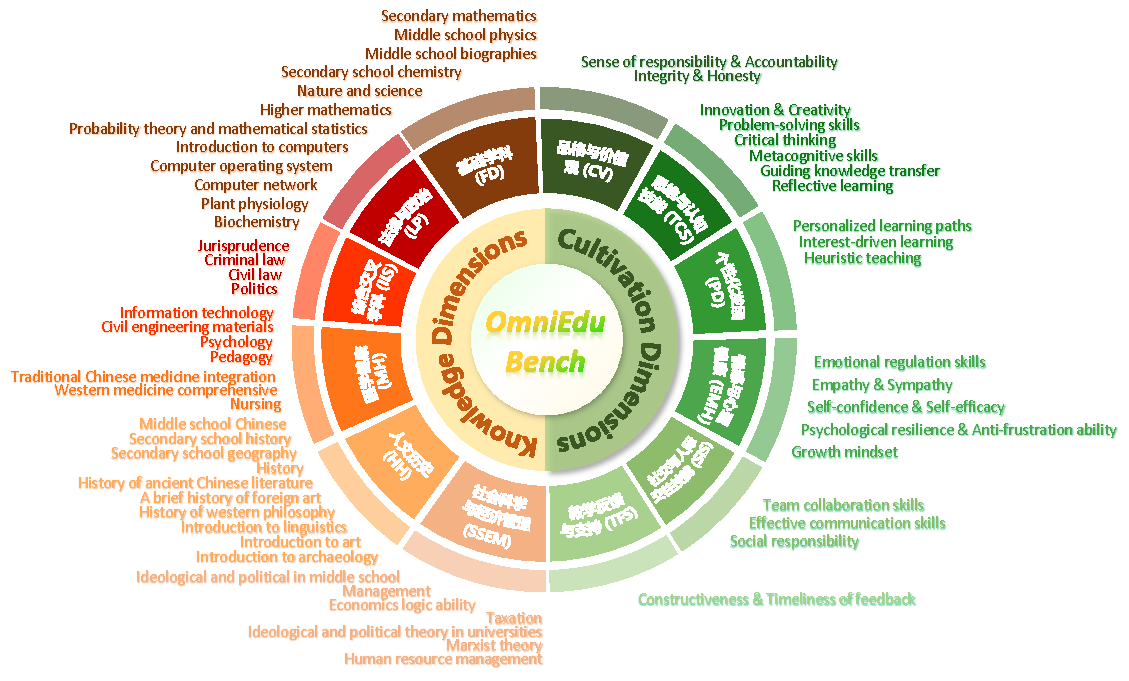
\includegraphics[height=0.6\textwidth]{figure/omniframe.pdf}
    \vspace{-8mm}
    \caption{Overview of OmniEduBench. The benchmark comprises two dimensions: 41 subjects across six categories in the knowledge, and 20 subjects across six categories in the cultivation.}
    \label{fig:omniframe}
    \vspace{-4mm}
\end{figure}
\section{OmniEduBench}

Our proposed OmniEduBench education benchmark is designed as a \textcolor{myorange}{natively Chinese education evaluation benchmark} that captures the unique linguistic and cultural knowledge of Chinese education, encompasses diverse question types, and assesses LLMs not only on their knowledge capabilities but also on the distinctive cultivation competencies required in real-world educational scenarios. 

\subsection{Task Definition}

\textbf{Knowledge dimension} focuses on evaluating the model’s mastery of subject-specific knowledge. Tasks in this dimension include 11 common exam question types (\textit{e.g.}, multiple choice, multiple answer, fill-in-the-blank, short answer, composite questions, term explanation, True/False, calculation, logical reasoning, case analysis, and essay). These 11 question types span a wide range of disciplines, from humanities and history to science, engineering, and professional fields. The primary goal is to assess the LLM’s problem-solving capabilities within the context of real-world education. 

\textbf{Cultivation dimension} assesses LLMs on their ability to support holistic educational objectives beyond mere knowledge acquisition. This includes guiding students’ thinking processes, fostering moral and value development, enhancing emotional understanding, and promoting critical reasoning skills. Tasks in this dimension are designed to reflect realistic learning scenarios, where models must provide pedagogically sound feedback that aligns with students’ cognitive and emotional needs.

\begin{figure}[tbp]
    \centering
    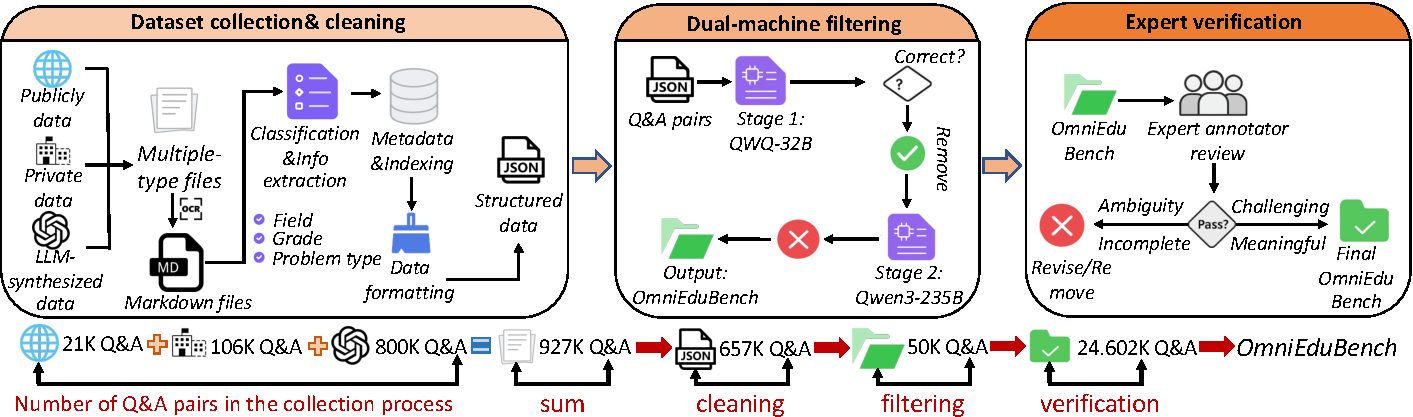
\includegraphics[height=0.3\textwidth]{figure/omniprocess.pdf}
    \vspace{-6mm}
    \caption{Overview of the construction process, including collection, cleaning, filtering, verification.}
    \label{fig:omniprocess}
    \vspace{-5mm}
\end{figure}

\subsection{Benchmark Construction}
\label{subsec:bc}

In this section, we provide a detailed overview of the construction process for the proposed OmniEduBench education evaluation benchmark, as illustrated in Figure~\ref{fig:omniprocess}. The process consists of four key stages: dataset collection, dataset cleaning, dual-machine filtering, and expert verification.

\textbf{Dataset collection.} OmniEduBench is designed to encompass a wide range of diverse scenarios to enable comprehensive evaluation. To achieve this, we employ three distinct data collection methods, carefully balancing diversity and efficiency in the construction of the OmniEduBench benchmark.

\textit{Manual collection of publicly available data.} 
Existing benchmarks often lack sufficient diversity in question types and knowledge coverage, making them inadequate for our 41 subjects in knowledge dimensions. To address this gap, we manually collected additional data from publicly available online resources (\textit{e.g.}, XuekeNet, ZujuanNet, ShijuanNet, ShitiNet) to enrich diversity and ensure coverage of underrepresented scenarios, such as primary and career education. Furthermore, guided by the Catalogue of Undergraduate Programs in Regular Higher Education Institutions~\footnote{\url{http://www.moe.gov.cn/srcsite/A08/moe_1034/s4930/202403/W020240319305498791768.pdf}} issued by China’s Ministry of Education, we curated a large body of review materials and exam questions across 13 academic disciplines, including philosophy, education, law, literature, history, science, engineering, agriculture, medicine, military science, management, and the arts. This effort significantly improves distributional balance and provides a more faithful reflection of real applications.

\textit{Manual collection of private data.}
Data contamination remains one of the most critical challenges in constructing evaluation datasets for LLMs. To mitigate this risk, we manually collected additional data from private resources, such as internal school exam papers. Unlike widely circulated national exams, these materials have never appeared on the public Internet or been included in large-scale web crawls, effectively reducing the risk of leakage. Incorporating such private data enhances the reliability and fairness of the benchmark, while providing a more rigorous assessment of models.

\textit{LLM-generated data.}
Given the difficulty of directly obtaining data in the cultivation dimension, we leveraged LLMs to generate a substantial number of scenario-based question–answer pairs, aiming to supplement gaps in existing resources. To ensure the quality of the synthetic data, we invited five education experts to conduct discussions on 20 cultivation subjects and consulted relevant books, papers, and other materials. The collected content was organized into a database, which was then provided to the LLM to enhance the fidelity and accuracy of the generated data. For generated questions, to increase their challenge, we designed highly confounding distractors via prompts and conducted sampling checks and revisions with expert verification (please see more details in expert verification). 
\textcolor{myorange}{Finally, we collected a total of 927K question–answer (Q\&A) pairs, including 21K from publicly available data, 106K from private data, and 800K generated by LLMs.}

\textbf{Dataset cleaning.}
The entire data cleaning process consists of multiple steps. (1) We used MinerU~\citep{wang2024mineru} to convert the collected 927K Q\&A pairs into Markdown (md) format, enabling structured management and efficient information extraction. (2) Detailed metadata were extracted for each question, including subject, grade level, question type, and knowledge tags, to construct comprehensive question profiles that facilitate data management and subsequent analysis. (3) Standard data cleaning procedures were applied, including deduplication, removal of questions with missing key content, filtering of sensitive or inappropriate content, and exclusion of questions that rely on external information.\textcolor{myorange}{After the cleaning process, we obtained a total of 657K Q\&A pairs.}

\begin{table}[tbp]
    \centering
    \caption{Statistics of OmniEduBench and more detailed per-subject information are shown in the Appendix. Bilingual names and abbreviations of six knowledge and six cultivation dimensions.}
    \vspace{0.2mm}
    \resizebox{0.99\textwidth}{!}{
    \begin{tabular}{lcc|lcc}
        \toprule
        \multicolumn{3}{c|}{\textcolor{myorange}{\textit{Knowledge dimension}}} & \multicolumn{3}{c}{\textcolor{myorange}{\textit{Cultivation dimension}}}\\
        English name & Abbreviation & Chinese name & English name & Abbreviation & Chinese name \\
        \midrule
        Law \& Politics  & LP &  \cc{法律与政治} & Character \& Values & CV & \cc{品格与价值观} \\ 
        Foundational Disciplines & FD & \cc{基础学科} & Personalized Development & PD & \cc{个性化发展} \\
        Humanities \& History & HH & \cc{人文与历史} & Social \& Interpersonal Skills & SIS & \cc{社会与人际交往} \\
        Medicine \& Health & MH & \cc{医学与健康}  & Thinking \& Cognitive Skills & TCS & \cc{思维与认知能力} \\
        Interdisciplinary \& Integrated Subjects & IIS & \cc{综合与交叉学科} &  Teaching Feedback \& Support & TFS & \cc{教学反馈与支持}) \\
        Social Sciences \& Economics Management & SSEM & \cc{社会科学与经济管理} & Emotional \& Mental Health & EMH & \cc{情感与心理健康} \\
        \bottomrule
    \end{tabular}}
%     \label{tab:name}
%     \vspace{-6mm}
% \end{table}
% \begin{table}[tbp]
%     \centering
%     \caption{Statistics of OmniEduBench with detailed per-subject information shown in the Appendix.}
%     \vspace{0.2mm}
    \resizebox{0.99\textwidth}{!}{
    \begin{tabular}{lcc|lcc|lcc}
        % \toprule
        Category & Subjects & Questions & Category & Subjects & Questions & Category & Subjects & Questions \\
        \midrule
        \multicolumn{3}{c|}{\textcolor{myorange}{\textit{In terms of dimension}}} & \multicolumn{3}{c|}{\textcolor{myorange}{\textit{In terms of Knowledge}}} & \multicolumn{3}{c}{\textcolor{myorange}{\textit{In terms of Cultivation}}} \\
        Knowledge  & 41 & 18,121 & LP & 4 & 1,455 & CV & 2 & 694 \\
        Cultivation & 20 & 6,481 & FD  & 11 & 7,918 & PD & 3 & 1,031 \\
        \multicolumn{3}{c|}{\textcolor{myorange}{\textit{In terms of different level}}} & HH & 10 & 5,331 & SIS & 3 & 736 \\
        K-12 Schools  & 10 & 4,384 & MH & 3 & 918 & TCS & 6 & 1,900 \\
        High school & 11 & 6,735 & IIS & 4 & 914 & TFS & 1 & 193 \\
        College  & 30 & 6,364 & SSEM & 9 & 1,643 & EMH & 5 & 1,833 \\
        \midrule
        Total  & 61 & 24,602 & Total  & 41 & 18,179 & Total  & 20 & 6,387 \\
        \bottomrule
    \end{tabular}}
    \label{tab:sta}
    \vspace{-6mm}
\end{table}

\textbf{Dual-machine filtering.}
To ensure OmniEduBench is a high-quality and challenging benchmark, we implemented a dual-model filtering mechanism on an \textcolor{myorange}{initial set of 657K Q\&A pairs}. Specifically, we first evaluated all questions using QWQ32B~\citep{qwq32b}, retaining only those that the model answered incorrectly. This initial filtering resulted in \textcolor{myorange}{a subset of 430K Q\&A pairs}. These questions then underwent a second filtering stage with the same strategy, this time using Qwen3-235B~\citep{yang2025qwen3}, ultimately yielding the final \textcolor{myorange}{set of 50K high-quality} and challenging data. 

\textbf{Expert verification.}
We recruited 50 master's students to perform an initial quality check on the dataset based on five predefined dimensions (as shown in Table~\ref{tab:ev}), removing any data that did not meet the criteria, which resulted in \textcolor{myorange}{a final set of 24.602K Q\&A pairs} for OmniEduBench. Subsequently, we invited 5 senior annotation experts to conduct a rigorous quality review on a 15\% random sample of the OmniEduBench. The review results, shown in Table~\ref{tab:ev}, indicate that the dataset maintains high overall quality, demonstrating both reliability and applicability.

\begin{table}[tbp]
    \centering
    \caption{Expert validation results for the OmniEduBench dataset.}
    \vspace{0.2mm}
    \resizebox{0.99\textwidth}{!}{
    \begin{tabular}{lcccc}
        \toprule
        Metric English name & Metric Chinese name & Average & Standard deviation & Inter-rater agreement  \\
        \midrule
        Overall quality & \cc{整体质量} & 4.8 & 0.1 & 0.90\\
        Clarity & \cc{问题清晰度} & 4.5 & 0.2 & 0.85 \\
        Option perplexity & \cc{选项困惑度} & 4.8 & 0.3 & 0.83 \\
        Accuracy & \cc{答案准确性} & 4.8 & 0.1 & 0.90 \\
        Cultivation value & \cc{育人价值} & 4.6 & 0.2 & 0.88 \\
        \bottomrule
    \end{tabular}}
    \label{tab:ev}
    \vspace{-6mm}
\end{table}

\subsection{Evaluation Criteria}
\label{subsec:ec}

Based on the characteristics of different question types, we adopt two evaluation metrics: (1) \textbf{Choice}. For questions with a standard answer, we directly evaluate the provided answer. This simplifies the scoring process, as the model only needs to select the most appropriate option, thereby reducing ambiguity in assessment. (2) \textbf{LLM-assisted scoring}. For short-answer questions that may have multiple valid forms but are semantically equivalent, we employ an LLM-assisted scoring method. This approach provides greater flexibility, avoids imposing unnecessary constraints on the model, and allows for a more accurate evaluation of the model’s semantic understanding and expression.

\subsection{Statistics}

Through rigorous data filtering and expert validation, we collected 18.121K high-quality question–answer pairs for the knowledge and 6.481K for the cultivation. As illustrated in Figure~\ref{fig:omniframe} and summarized in Table~\ref{tab:sta}, with more detailed per-subject statistics provided in the Appendix, the dataset spans 12 major categories, as shown in Table~\ref{tab:sta}, including K-12, higher school, university-level courses, and cultivation aspects such as emotion and reasoning, covering a total of 61 specific scenarios. Figures~\ref{fig:omni12} and~\ref{fig:omni34} present some representative examples in different dimensions and question types. The questions exhibit wide variability in type and difficulty and are sourced from diverse origins, primarily newly collected from public or private resources or manually constructed. 

\begin{figure}[tbp]
    \centering
    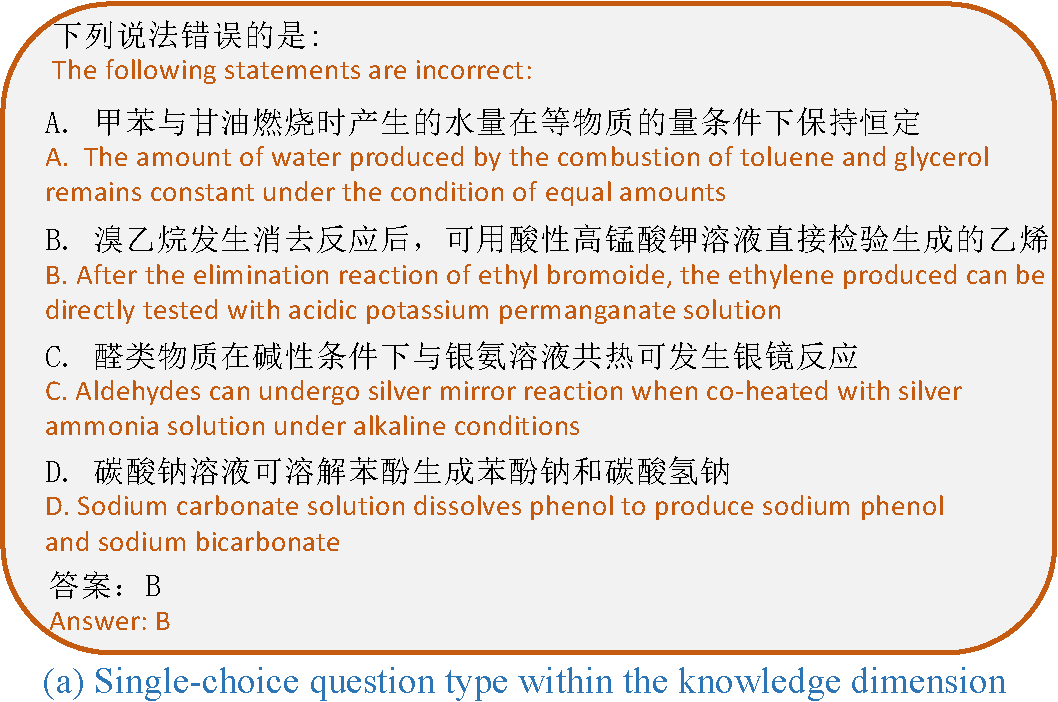
\includegraphics[height=0.32\textwidth]{figure/omni1.pdf}
    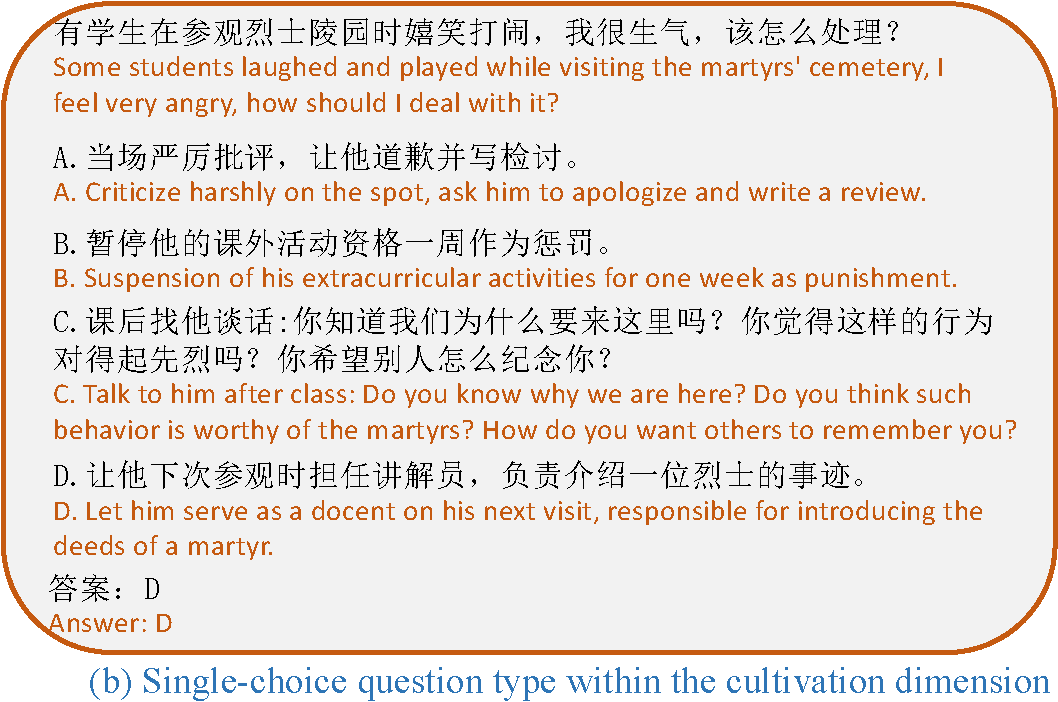
\includegraphics[height=0.32\textwidth]{figure/omni2.pdf}
    \vspace{-3mm}
    \caption{Example of (a) a single-choice question in the knowledge from a college chemist. (b) A single-choice question in the cultivation. English translations are shown for better readability.}
    \label{fig:omni12}
    \vspace{-3mm}
\end{figure}

\begin{figure}[tbp]
    \centering
    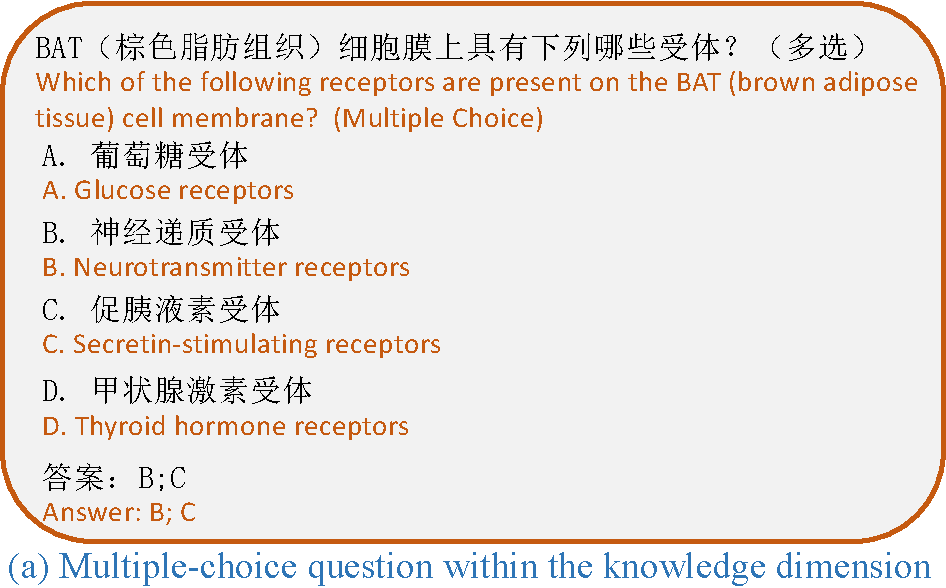
\includegraphics[height=0.3\textwidth]{figure/omni3.pdf}
    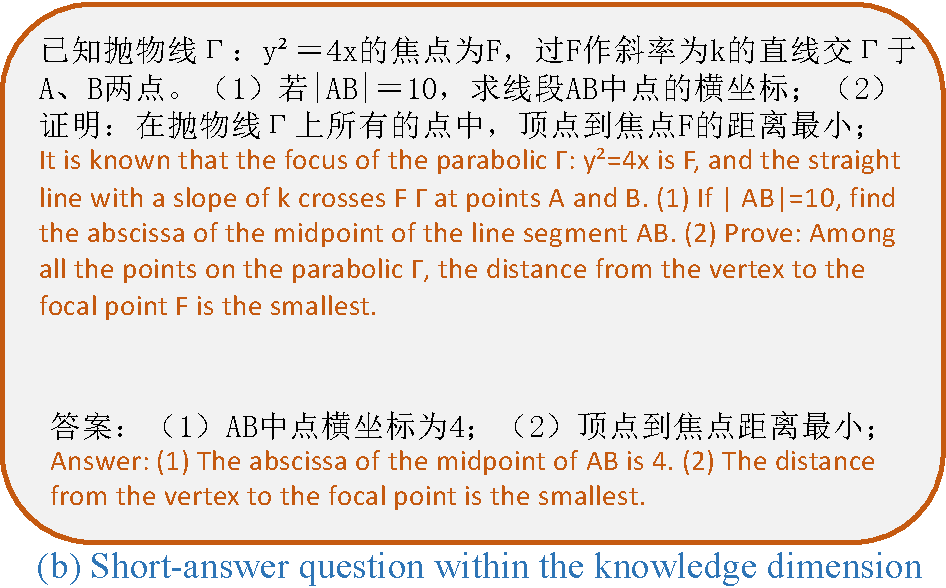
\includegraphics[height=0.3\textwidth]{figure/omni4.pdf}
    \vspace{-3mm}
    \caption{Example of (a) a multiple-choice question in the knowledge from Biology. (b) A short-answer question in the knowledge from Math. English translations are shown for better readability.}
    \label{fig:omni34}
    \vspace{-3mm}
\end{figure}





%%%基础教育
%在本研究中,我们首先通过在互联网上爬取和收集大量 K12 阶段的考试试卷,建立了一个较为完整的题库。为了便于后续处理和编辑,这些试卷数据经过 minerU 工具转化为 Markdown (md) 格式,从而实现结构化管理与信息的高效提取。

%在数据预处理环节,我们进一步对题目进行了分类与信息抽取,为每道题打上了多维度标签,包括 科目、学段以及题目类别。这一过程不仅使得题目能够更清晰地组织和索引,同时也为后续的数据分析与模型训练提供了必要的元信息支撑。

%为了保证题目的完整性与适用性,我们引入了 关键词过滤机制,用于检测题目及其对应解答是否依赖额外信息。例如,由于本研究所构建的数据集为单模态文本数据,并不包含图片信息,因此部分题目若在解答过程中需要图像、图表或公式等外部信息,则会通过关键词检索加以识别与剔除。这一策略有效降低了由于信息缺失而导致的题目不合理性。

%在构建题目与答案对应关系的过程中,我们利用 生成式大语言模型 (LLM) 对题目进行自动化解答匹配。然而,考虑到大模型在推理过程中存在一定的不确定性,其生成的答案可能与题意不符,甚至存在逻辑错误或事实性错误。为此,我们在后处理阶段引入了 闭源大模型作为校验器,对生成的题目与答案进行准确性和合理性检测,从而过滤掉了大量不符合标准的匹配结果。通过这一多层次的筛选流程,我们有效提升了数据集的质量与可靠性。

%整体而言,本研究构建的处理管线包括:数据爬取 → 格式转化 → 分类标注 → 关键词过滤 → 答案生成 → 准确性验证与筛选。这一系统化流程不仅确保了题目数据的规范性和科学性,同时也为后续的教育应用、智能出题与自动批改等场景奠定了坚实的基础。


%育人属性

%为系统评估生成式大语言模型(LLM)在 K12 场景下对关键“育人属性”的理解与迁移能力,本文基于公开可获得的教育类图书与学术论文构建场景化问答数据与相应评测协议。研究目标在于检验模型能否在真实教育情境中作出与价值导向一致、具有可执行性的判断与决策,而非仅停留在术语识别或模板化应答层面。

%数据构建首先从互联网收集与“育人”主题相关的书籍和论文,并对原始文本进行去重、清洗与结构化处理。在此基础上,提取“定义性描述”“干预策略与做法”“正反面案例”“可观察行为指标”等证据片段,形成可控生成所依托的素材池。随后依据“能力—情境—策略—行为表现”等维度对语料进行主题聚类,既保证内容的理论锚定与可追溯性,又为后续的场景重写与题项约束提供精确的证据支撑。

%在理论梳理和语料校对的基础上,本文将“育人”维度划分为二十个可操作属性:成长型思维、创新与创造力、反馈的建设性与及时性、反思性学习引导、个性化学习路径、批判性思维、情绪调控能力、启发式教学、社会责任感、同理心与共情、团队协作能力、问题解决能力、兴趣驱动学习、心理韧性与抗挫力、有效沟通能力、元认知能力、责任感与担当、正直与诚信、知识迁移能力、自信心与自我效能感。每个属性均提供简要定义、典型正向行为表现、易混淆的邻近概念与误用情形,以及可迁移的应用情境(课堂、家庭、社团、线上协作等),以此作为题项生成与评价的明确锚点。

%题项生成采用“证据驱动的场景重写—问项生成—答案约束”的流程。首先构建情境原型,明确角色(教师/学生/家长/同伴)、环境(学科或活动类型、线上/线下)、约束(时间、资源、评价压力)与目标(认知、情感、社会性)。其次完成属性对齐,为每个场景设定一个主属性及一至两个次属性,并在题干中避免显式暴露属性名称以减少词面提示与启发效应。随后指引 LLM 在限定的证据片段内生成题干、标准答案与简短判据,使答案体现“策略—因果链—预期结果”的可执行性与场景一致性,同时根据小学/初中/高中进行词汇难度与社会情境复杂度的年段适配。鉴于本研究数据为单模态文本形态,题项设计不依赖图片或图表信息,确保在无外部多模态资源时亦可完成作答。

%为检验模型对属性内涵的真正理解,本文为每个题项系统设计高迷惑度干扰项。干扰项刻意呈现“表层合理但情境失配”的特征,或在概念上与目标属性邻近却在要义上偏离(如反馈缺乏具体性或时效性),亦或提供短期有效但长期失衡的做法(例如立竿见影却削弱内在动机、诚信或协作),并在必要时设置触及教育伦理与安全红线的选项用于价值底线辨识。通过这类“部分正确但不符合场景”的设定,评测能够区分术语命中与真正理解。

%质量控制采取自动与人工相结合的策略。自动化阶段使用闭源校验模型对“题干—标准答案—理据”的一致性与价值合规性进行审查,剔除逻辑断裂与价值冲突样本,同时开展关键词泄露检测以避免目标属性或强提示词出现在题干中。必要时辅以具教育背景的人审抽检,对样本进行“一致/存疑/剔除”的标注并统计一致性指标;在试测基础上对题项进行难度标定,形成易/中/难分层,既便于后续实验设计,也有助于分析模型在不同难度水平上的表现差异。

%评测协议以多项选择题为载体,采用准确率作为核心指标,并以“标准答案与最强干扰项间的胜率差”衡量区分度,以检验干扰项的有效性与题项的辨析力。在模型可提供置信度的情况下,进一步计算 Brier 分数或期望校准误差以评估校准度。除总体结果外,报告分属性表现与跨场景的一致性,以检验模型在不同教育情境中的鲁棒性,并对各属性的题量、难度与通过率进行分布均衡性分析,防止由数据分布不均带来的结论偏置。

%该方案与本文前述的学科题库处理流水线保持兼容:从爬取与格式转化、分类标注、关键词过滤,到题目—答案的生成与闭源模型校验,均可复用统一的工程化组件。所有样本均绑定属性标签、年段、场景与角色等元数据,以支持高效检索与细粒度分析。研究全程遵循未成年人保护原则与学术伦理规范,避免刻板印象与歧视性表述;对于涉及心理与情绪的情境采用非伤害性语言;在数据使用与发布环节遵从版权与引用要求,尽可能实施最小必要摘录与重写,并移除可识别个人信息,同时对价值判断标准的理论来源予以说明,以提升研究的透明度与可复现性。


% 高等教育数据集处理过程
% 基于我们的调研,在目前的公开数据集中,中国高等教育习题的数据是广泛欠缺的。我们参照中国教育部普通高等学校本科专业目录,收集了涵盖哲学、教育学、法学、教育学、文学、历史学、理学、工学、农学、医学、军事学、管理学、艺术学这十三个学科大类的大量的中国高等教育复习资料、考研习题,并整理形成了我们的数据集。然而,这些习题大部分以PDF的形式存在,我们借助了MinerU提取工具从中解析出文字,并整理形成我们的高等教育题目数据集。为了保证题目的质量,我们进行了人工质检,筛除掉了识别混乱、语义不过关的题目。同时,为了确保题目的难度,我们采用了开源模型(Qwen-72B)进行了一轮答题,仅筛选了Qwen-72B答错并认为有挑战性的题目,以此保证了数据集中的题目对于大语言模型而言,是非常具有挑战性的。

% [1] 中国教育部普通高等学校本科专业目录:http://www.moe.gov.cn/srcsite/A08/moe_1034/s4930/202403/W020240319305498791768.pdf
% [2]MinerU: An Open-Source Solution for Precise Document Content Extraction 
% (https://arxiv.org/abs/2409.18839)


\section{Experiments}

In this section, we evaluate the performance of state-of-the-art (SOTA) methods in both English and Chinese. The experimental results indicate that OmniEduBench remains a competitive benchmark.

\subsection{Experimental Setup}

\begin{table}[t]
    \centering
    \caption{Zero-shot average accuracy (\%) across six categories in the \textbf{knowledge}. The highest accuracy is \textbf{bold}, and the second highest is \underline{underlined}. More results are provided in the Appendix.}
    \vspace{0.2mm}
    \resizebox{0.99\textwidth}{!}{
        \begin{tabular}{lccc|cccccc|c}
            \toprule
            \textbf{Model} & \textbf{Parameters} & \textbf{Access} & \textbf{Creator} & \textbf{FD} & \textbf{HH} & \textbf{SSEM} & \textbf{LP} & \textbf{MH} & \textbf{IIS} & \textbf{Average} \\ \midrule
            Qwen3  & 8B & Weights & Alibaba & 53.02 & 38.53 & 36.58 & 30.17 & 36.71 & 37.75 & 43.86 \\
            Qwen3   & 14B & Weights & Alibaba & 36.32 & 36.78 & 35.12 & 27.29 & 36.82 & 35.67 & 35.62 \\
            MuduoLLM & 14B & Weights & BNU \& TAL & 28.20 & 40.82 & 32.99 & 36.15 & 39.11 & 31.40 & 33.68 \\
            QwQ   & 32B & Weights & Alibaba & \underline{61.25} & 48.51 & 42.24 & \underline{49.90} & 55.01 & 47.26 & \underline{53.87} \\
            Seed-OSS     & 36B & Weights & ByteDance & 48.81 & \underline{50.14} & \underline{45.34} & 48.66 & \textbf{61.00} & \underline{49.56} & 49.53 \\
            Qwen2.5 & 72B & Weights & Alibaba & 19.53 & 30.95 & 20.57 & 13.26 & 23.86 & 20.90 & 22.76 \\
            Qwen3   & 235B (22B active) & Weights & Alibaba & 34.24 & 47.01 & 36.21 & 44.26 & 58.71 & 46.61 & 40.82 \\
            DeepSeek-V3.1 & 671B (37B active) & Weights & DeepSeek & 31.65 & 40.65 & 35.00 & 29.42 & 50.54 & 45.19 & 36.05 \\
            \midrule
            GPT-4o  & Undisclosed & API & OpenAI & 21.15 & 26.94 & 23.92 & 22.13 & 34.75 & 27.13 & 24.17 \\
            Claude-4 Sonnet  & Undisclosed & API & Anthropic & 41.49 & 44.29 & 35.36 & 27.56 & 34.86 & 42.34 & 40.35 \\
            Gemini-2.5 Pro  & Undisclosed & API & Google & \textbf{73.83} & \textbf{55.13} & \textbf{46.68} & \textbf{55.40} & \underline{60.68} & \textbf{54.16} & \textbf{62.76} \\
            \bottomrule
        \end{tabular}}
    \label{tab:main_results_kd}
    \vspace{-5.6mm}
\end{table}

\begin{table}[tbp]
    \centering
    \caption{Zero-shot average accuracy (\%) across six categories in the \textbf{cultivation}. The highest accuracy is \textbf{bold}, and the second highest is \underline{underlined}. More results are provided in the Appendix.}
    \vspace{0.2mm}
    \resizebox{0.99\textwidth}{!}{
        \begin{tabular}{lccc|cccccc|c}
            \toprule
            \textbf{Model} & \textbf{Parameters} & \textbf{Access} & \textbf{Creator} & \textbf{TCS} & \textbf{EMH} & \textbf{SIS} & \textbf{CV} & \textbf{PD} & \textbf{TFS} & \textbf{Average} \\ \midrule
            Qwen3 & 8B & Weights & Alibaba  & 70.95 & 66.67 & 69.16 & 62.25 & 70.13 & \textbf{77.20} & 68.62 \\
            Qwen3  & 14B & Weights & Alibaba & 67.79 & 60.77 & 63.72 & 56.20 & 64.31 & 71.50 & 63.60 \\
            MuduoLLM  & 14B & Weights & BNU \& TAL & 64.42 & 60.77 & 63.45 & \textbf{66.14} & 67.51 & 64.77 & 63.96 \\
            QwQ & 32B &Weights & Alibaba  & \textbf{73.16} & \underline{68.36} & 69.84 & 65.13 & \textbf{71.77} & \underline{72.02} & \textbf{70.27} \\
            Seed\mbox{-}OSS & 36B &Weights & ByteDance & 70.74 & 65.30 & 66.03 & 62.82 & 67.12 & 70.47 & 67.18 \\
            Qwen2.5 & 72B &Weights & Alibaba  & 67.89 & 64.38 & 65.62 & 59.51 & 65.57 & 67.88 & 65.34 \\
            Qwen3 & 235B (22B active) &Weights & Alibaba & 67.84 & 61.10 & 64.54 & 55.76 & 64.40 & 70.47 & 63.74 \\
            DeepSeek\mbox{-}V3.1  & 671B (37B active) &Weights& DeepSeek & 71.58 & 65.41 & 69.02 & 61.96 & \underline{71.00} & \textbf{77.20} & 68.55 \\
            \midrule
            GPT\mbox{-}4o & Undisclosed & API & OpenAI & 61.63 & 59.57 & 59.24 & 55.33 & 57.71 & 65.80 & 59.57 \\
            Claude\mbox{-}4\mbox{-}sonnet  & Undisclosed & API & Anthropic        & 71.95 & \textbf{70.05} & \textbf{70.92} & 64.55 & 69.25 & 71.50 & \underline{70.03} \\
            Gemini\mbox{-}2.5\mbox{-}pro & Undisclosed & API & Google      & \underline{72.26} & 66.07 & \underline{70.79} & \underline{65.71} & 70.32 & 67.36 & 69.14 \\
            \bottomrule
        \end{tabular}}
    \label{tab:main_results_cd}
    \vspace{-6mm}
\end{table}

\textbf{Baselines.}
We evaluate 11 mainstream large language models (LLMs) in total, including 3 cutting-edge closed-source models and 8 open-source models, one of which is a newly released education-oriented model. The closed-source models are GPT-4o~\citep{hurst2024gpt-4o}, Gemini-2.5 Pro~\citep{comanici2025gemini}, and Claude-4 Sonnet~\citep{claude4sonnet}. For the open-source models, we consider two main factors. First, they are grouped by parameter size into small (8B), medium (14B/32B/36B), and large (72B/235B/671B) scales. Second, they are categorized by functionality into: (a) general instruction-following models (Qwen2.5~\citep{qwen2.5}, Qwen3~\citep{yang2025qwen3}); (b) general reasoning models (QwQ~\citep{qwq32b}, Seed-OSS~\citep{seed2025seed-oss}, DeepSeek-V3.1~\citep{liu2024deepseek-v3}); and (c) education-specific models (MuduoLLM~\citep{muduollm2025}).

\textbf{Implementation details.}
In our experimental setup, we evaluate all large language models under both zero-shot and few-shot settings, with few-shot examples (0-, 1-, 3-, and 5-shot) drawn from a separately partitioned development set, distinct from the evaluation set. All open-source models are run using their official code, while closed-source models are accessed via official APIs. We consistently use Gemini-2.5 Pro as the LLM-assisted scoring model, unless otherwise specified.

\subsection{Main Results}

We evaluated all baseline models on OmniEduBench, reporting both per-task category and overall accuracy, as shown in Tables~\ref{tab:main_results_kd} and~\ref{tab:main_results_cd}). Results show that in the knowledge dimension, Gemini-2.5 Pro achieves the highest accuracy at 62.78\%, while in the cultivation dimension, the reasoning-enhanced version of QWQ performs best with an accuracy of 70.27\%. This performance highlights the challenging nature and strong discriminative power of the constructed OmniEduBench.

In the knowledge dimension, it is evident that, except for Gemini-2.5 Pro, closed-source models generally perform worse than open-source models on our OmniEduBench. For example, GPT-4o achieves an accuracy of 24.17\%, far below that of Qwen3-8B. This may indicate that the GPT series has relatively weak robustness when handling Chinese education exam-style questions. Meanwhile, model architecture has a significant impact on performance, such as Seed-OOS outperforms the Qwen family by more than 10\%. In the cultivation dimension, models generally perform better than in the knowledge dimension, which may be due to the fact that the cultivation tasks mainly consist of multiple-choice questions, making them simpler compared to knowledge tasks with 11 common exam question types. However, differences in performance between different model architectures still exist. Overall, GPT-40 performs the worst in both dimensions, with accuracy largely concentrated around 59.57\%, possibly because it has not been specifically optimized for this dimension.

\subsection{Analysis and Findings}

In this section, we further conduct extensive experiments at multiple levels, including few-shot examples, OmniEduBench HARD, and various LLM-assisted scoring methods.

\textbf{Results in few-shot examples.} In Table~\ref{tab:few-shot_kd}, we present in-context experimental results using different numbers of shots. As the number of shots increases, model performance generally improves; however, the overall gain is limited when considering the average results. We speculate that the drop in accuracy for some models is due to the fact that they have not (or not appropriately) incorporated few-shot examples during the instruction tuning stage. These findings suggest that while few-shot prompting can be beneficial for certain models, its effectiveness strongly depends on the model’s pretraining and instruction tuning strategies. Moreover, the limited average improvement indicates that simply increasing the number of shots may not always lead to substantial gains, highlighting the need for more sophisticated methods to integrate few-shot examples effectively. 

\begin{table}[tbp]
    \centering
    \caption{Average accuracy (\%) across six categories in one-shot, three-shot, and five-shot settings for the knowledge dimension. The highest accuracy is \textbf{bold}, and the second highest is \underline{underlined}.}
    \vspace{0.2mm}
    \resizebox{0.99\textwidth}{!}{
        \begin{tabular}{lccc|cccccc|c}
            \toprule
            \textbf{Model} & \textbf{Parameters} & \textbf{Access} & \textbf{Creator} & \textbf{FD} & \textbf{HH} & \textbf{SSEM} & \textbf{LP} & \textbf{MH} & \textbf{IIS} & \textbf{Average} \\ \midrule
            \multicolumn{11}{c}{\textcolor{myorange}{\textit{One-shot setting}}} \\
            Qwen3 & 8B & Weights & Alibaba & \textbf{52.80} & 46.45 & \textbf{41.90} & 29.76 & 40.20 & 40.59 & \textbf{41.95} \\
            MuduoLLM & 14B & Weights & BNU \& TAL & 27.36 & \underline{47.79} & 36.72 & 34.98 & 40.74 & 34.35 & 36.99 \\
            Qwen2.5 & 72B & Weights & Alibaba & 21.42 & 40.43 & 27.04 & 20.96 & 28.10 & 22.65 & 26.77 \\
            Qwen3 & 235B (22B activate) & Weights & Alibaba & \underline{37.72} & \textbf{60.79} & \underline{44.03} & \textbf{45.77} & \textbf{59.59} & \textbf{54.05} & \textbf{50.12} \\
            DeepSeek-V3.1 & 671B (37B activate) & Weights & DeepSeek & 30.00 & 41.73 & 34.65 & 30.72 & \underline{49.67} & 42.12 & \underline{38.15} \\
            \midrule
            \multicolumn{11}{c}{\textcolor{myorange}{\textit{Three-shot setting}}} \\
            Qwen3 & 8B & Weights & Alibaba & \textbf{52.98} & 46.00 & \textbf{39.74} & 30.65 & 39.32 & 40.85 & \underline{41.59} \\
            MuduoLLM & 14B & Weights & BNU \& TAL & 27.32 & \underline{46.86} & 35.79 & 33.81 & 39.54 & 32.42 & 35.96 \\
            Qwen2.5 & 72B & Weights & Alibaba & 21.43 & 40.86 & 27.27 & 20.41 & 27.12 & 23.88 & 26.83 \\
            Qwen3 & 235B (22B activate) & Weights & Alibaba & \underline{37.52} & \textbf{60.70} & \underline{43.40} & \textbf{45.77} & \textbf{59.48} & \textbf{52.57} & \textbf{49.54} \\
            DeepSeek-V3.1 & 671B (37B activate) & Weights & DeepSeek & 29.09 & 41.42 & 34.02 & 28.59 & \underline{48.80} & \underline{42.06} & 37.33 \\
            \midrule
            \multicolumn{11}{c}{\textcolor{myorange}{\textit{Five-shot setting}}} \\
            Qwen3 & 8B & Weights & Alibaba & \textbf{56.86} & 46.70 & \textbf{39.44} & 30.65 & 38.24 & 42.23 & \underline{42.35} \\
            MuduoLLM & 14B & Weights & BNU \& TAL & 26.93 & \underline{46.57} & 36.28 & 35.74 & 39.11 & 34.57 & 36.53 \\
            Qwen2.5 & 72B & Weights & Alibaba & 21.46 & 41.19 & 26.96 & 20.82 & 26.03 & 28.56 & 27.50 \\
            Qwen3 & 235B (22B activate) & Weights & Alibaba & \underline{37.40} & \textbf{60.41} & \underline{44.13} & \textbf{45.77} & \textbf{58.61} & \textbf{55.58} & \textbf{50.32} \\
            DeepSeek-V3.1 & 671B (37B activate) & Weights & DeepSeek & 29.39 & 41.17 & 32.87 & 28.45 & \underline{47.49} & 38.95 & 36.39 \\
            \bottomrule
        \end{tabular}}
    \label{tab:few-shot_kd}
\end{table}

\textbf{Results on OmniEduBench HARD.} In Figures~\ref{fig:omnihard_kd} and~\ref{fig:omnihard_cd}, we present the average accuracy of each model on OmniEduBench HARD. OmniEduBench HARD is a subset of OmniEduBench, consisting of the bottom 26\% of samples based on model performance, including approximately 1.552K cultivation samples and 7.620K knowledge samples, for a total of 9.172K examples. The experimental results show that: (1) all 11 LLMs exhibit a significant performance drop on OmniEduBench HARD, with even the best-performing model, Gemini, achieving less than 50\% accuracy; (2) Qwen2.5-72 performs the worst, significantly lower than the other models, indicating limited capability in handling difficult samples. These findings indicate that further research is needed to enhance LLMs’ ability to generalize and maintain high performance on hard subsets of educational benchmarks.

\begin{figure}[tbp]
    \centering
    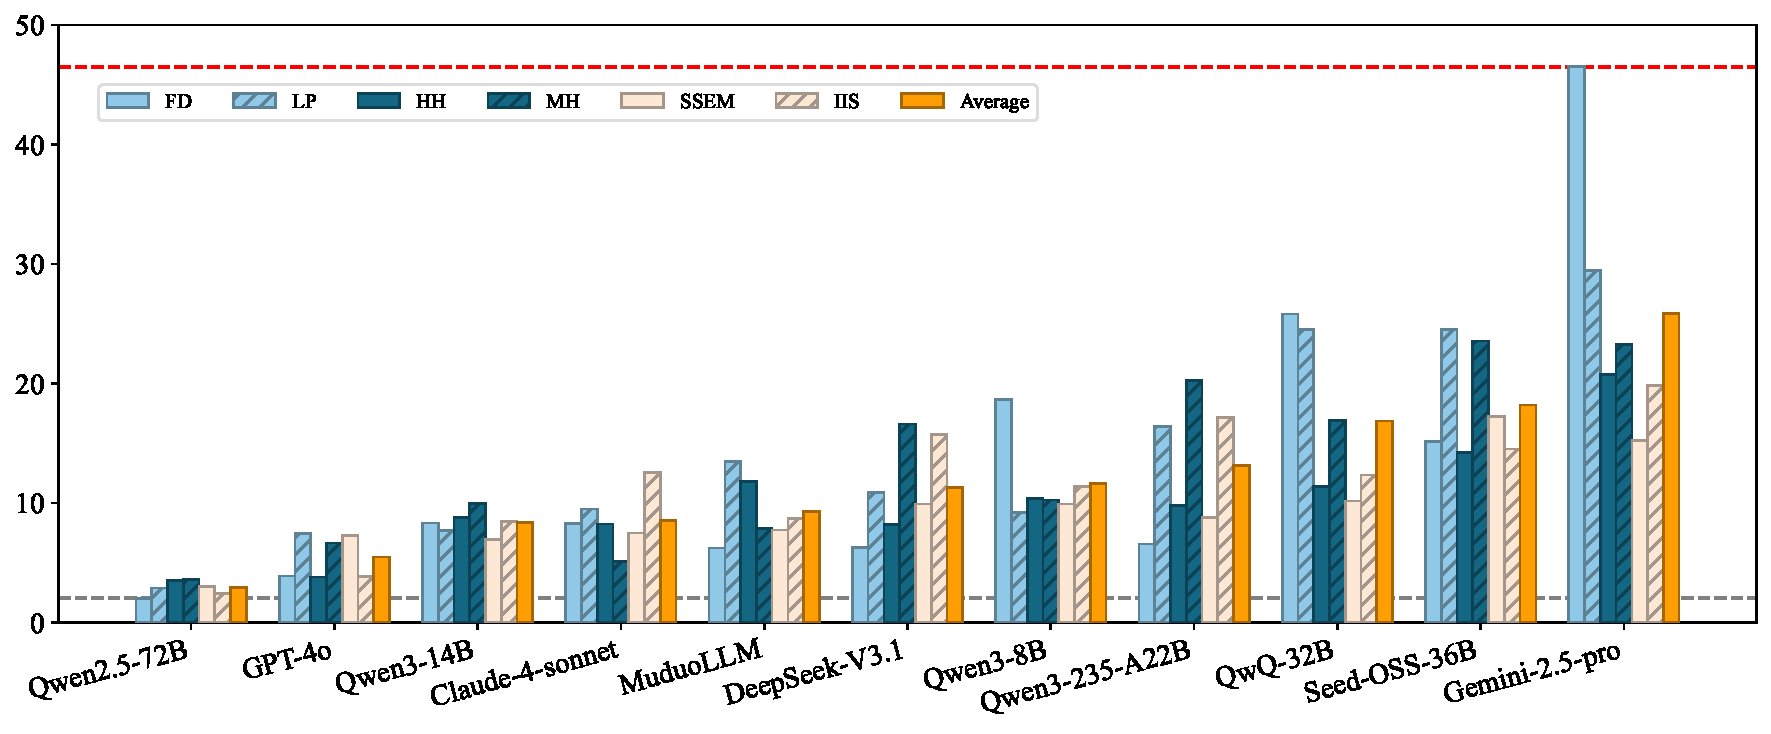
\includegraphics[height=0.41\textwidth]{figure/omnihardkd.pdf}
    \vspace{-5mm}
    \caption{Zero-shot average accuracy (\%) on the knowledge  dimension of OmniEduBench HARD.}
    \label{fig:omnihard_kd}
    \vspace{-3mm}
\end{figure}

\begin{figure}[tbp]
    \centering
    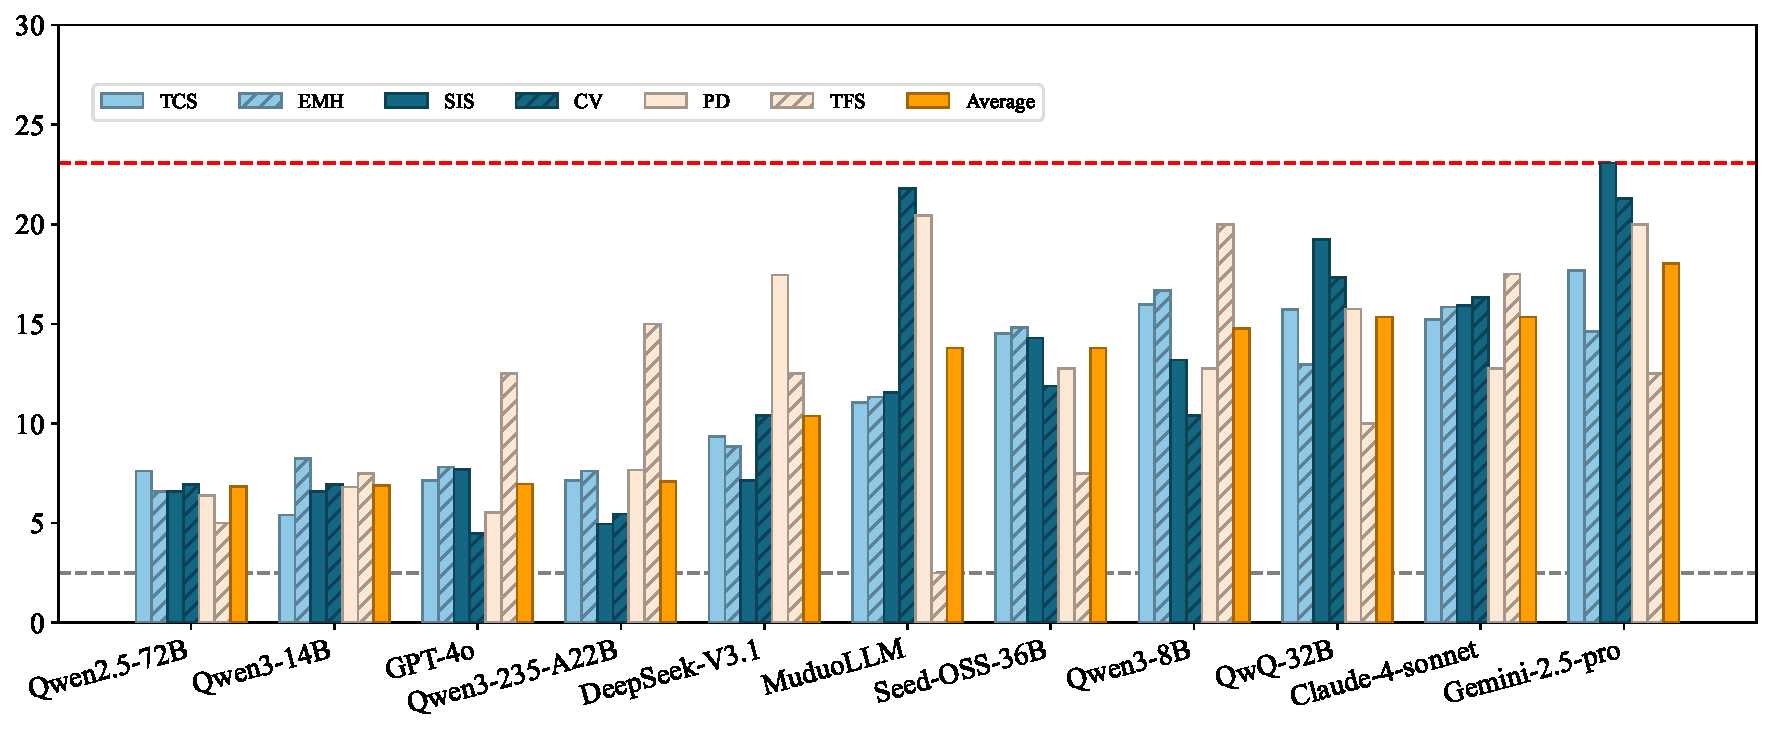
\includegraphics[height=0.41\textwidth]{figure/omnihardcd.pdf}
    \vspace{-5mm}
    \caption{Zero-shot average accuracy (\%) on the cultivation  dimension of OmniEduBench HARD.}
    \label{fig:omnihard_cd}
    \vspace{-3mm}
\end{figure}

\textbf{Results using different LLM-assisted scoring methods.}
In Table~\ref{tab:main_results_kd_llms}, we present the experimental results using different LLM-assisted scoring methods. The performance of the scoring model directly affects the evaluation outcomes: higher-quality scoring models provide more accurate assessments, leading to more precise measurements of the evaluated models’ capabilities. In this study, we employed three scoring models of varying quality. Overall, GPT-4o performed relatively poorly as a scoring model, failing to accurately evaluate the responses of LLMs. Consequently, the overall effectiveness of LLM-assisted evaluation is reduced when GPT-4o is used, highlighting the critical importance of selecting high-quality scoring models to ensure accurate and meaningful assessments. These findings suggest that the choice of scoring model can substantially influence the perceived performance of evaluated LLMs, and careful selection of scoring models is necessary.

\begin{table}[tbp]
    \centering
    \caption{Zero-shot average accuracy (\%) across six categories in the knowledge using different LLM-assisted scoring methods. The highest accuracy is \textbf{bold}, and the second highest is \underline{underlined}.}
    \vspace{0.2mm}
    \resizebox{0.99\textwidth}{!}{
        \begin{tabular}{lccc|cccccc|c}
            \toprule
            \textbf{Model} & \textbf{Parameters} & \textbf{Access} & \textbf{Creator} & \textbf{FD} & \textbf{HH} & \textbf{SSEM} & \textbf{LP} & \textbf{MH} & \textbf{IIS} & \textbf{Average} \\ \midrule
            \multicolumn{11}{c}{\textcolor{myorange}{\textit{Qwen3-A235B-assisted scoring method~\citep{yang2025qwen3}}}} \\
% Qwen3  & 8B & Weights & Alibaba & 55.45 & 48.51 & 42.54 & 30.86 & 38.13 & 44.42 & 48.85 \\
% Qwen3   & 14B & Weights & Alibaba & 37.82 & 48.70 & 40.60 & 29.07 & 38.45 & 41.14 & 40.76 \\
% MuduoLLM & 14B & Weights & BNU \& TAL & 27.78 & 43.22 & 34.08 & 36.01 & 39.00 & 29.21 & 34.18 \\
QwQ   & 32B & Weights& Alibaba & \underline{61.26} & 55.82 & 45.22 & \underline{50.10} & 55.66 & 48.36 & \underline{56.39} \\
Seed-OSS     & 36B &Weights & ByteDance & 51.16 & \underline{63.04} & \underline{51.55} & 50.38 & \textbf{62.31} & \underline{57.33} & 55.49 \\
% Qwen2.5 & 72B & Weights& Alibaba & 21.05 & 40.90 & 25.62 & 14.71 & 25.93 & 22.21 & 27.08 \\
% Qwen3   & 235B (22B active) & Weights & Alibaba & 37.11 & 59.20 & 42.97 & 45.77 & 61.00 & 53.61 & 46.85 \\
% DeepSeek-V3.1 & 671B (37B active) &Weights & DeepSeek & 29.94 & 40.47 & 33.72 & 29.42 & 50.33 & 41.36 & 34.93 \\
GPT-4o  & Undisclosed & API & OpenAI & 23.59 & 36.77 & 28.79 & 23.92 & 35.73 & 31.40 & 28.96 \\
Claude-4 Sonnet  & Undisclosed & API & Anthropic & 43.54 & 55.52 & 40.47 & 27.77 & 36.17 & 47.48 & 45.34 \\
Gemini-2.5 Pro  & Undisclosed & API & Google & \textbf{75.01} & \textbf{65.67} & \textbf{52.95} & \textbf{56.29} & \underline{61.44} & \textbf{61.49} & \textbf{67.41} \\
            \midrule
            \multicolumn{11}{c}{\textcolor{myorange}{\textit{Gemini-2.5 Pro-assisted scoring method~\citep{comanici2025gemini}}}} \\
% Qwen3  & 8B & Weights & Alibaba & 53.02 & 38.53 & 36.58 & 30.17 & 36.71 & 37.75 & 43.86 \\
% Qwen3   & 14B & Weights & Alibaba & 36.32 & 36.78 & 35.12 & 27.29 & 36.82 & 35.67 & 35.62 \\
% MuduoLLM & 14B & Weights & BNU \& TAL & 28.20 & 40.82 & 32.99 & 36.15 & 39.11 & 31.40 & 33.68 \\
QwQ   & 32B & Weights& Alibaba & \underline{61.25} & 48.51 & 42.24 & \underline{49.90} & 55.01 & 47.26 & \underline{53.87} \\
Seed-OSS     & 36B &Weights & ByteDance & 48.81 &\underline{50.14} & \underline{45.34} & 48.66 & \textbf{61.00} &\underline{49.56} & 49.53 \\
% Qwen2.5 & 72B & Weights& Alibaba & 19.53 & 30.95 & 20.57 & 13.26 & 23.86 & 20.90 & 22.76 \\
% Qwen3   & 235B (22B active) & Weights & Alibaba & 34.24 & 47.01 & 36.21 & 44.26 & 58.71 & 46.61 & 40.82 \\
% DeepSeek-V3.1 & 671B (37B active) &Weights & DeepSeek & 31.65 & 40.65 & 35.00 & 29.42 & 50.54 & 45.19 & 36.05 \\
GPT-4o  & Undisclosed & API & OpenAI & 21.15 & 26.94 & 23.92 & 22.13 & 34.75 & 27.13 & 24.17 \\
Claude-4 Sonnet  & Undisclosed & API & Anthropic & 41.49 & 44.29 & 35.36 & 27.56 & 34.86 & 42.34 & 40.35 \\
Gemini-2.5 Pro  & Undisclosed & API & Google & \textbf{73.83} & \textbf{55.13} & \textbf{46.68} & \textbf{55.40} & \underline{60.68} & \textbf{54.16} & \textbf{62.76} \\
            \midrule
            \multicolumn{11}{c}{\textcolor{myorange}{\textit{GPT-4o-assisted scoring method~\citep{hurst2024gpt-4o}}}} \\
% Qwen3  & 8B & Weights & Alibaba & 51.65 & 35.38 & 33.60 & 31.00 & 37.36 & 31.18 & 41.84 \\
% Qwen3   & 14B & Weights & Alibaba & 34.61 & 34.86 & 31.89 & 27.77 & 36.49 & 28.34 & 33.67 \\
% MuduoLLM & 14B & Weights & BNU \& TAL & 27.68 & 36.68 & 30.13 & 35.88 & 38.78 & 26.81 & 31.71 \\
QwQ   & 32B & Weights& Alibaba & \underline{56.61} & 42.87 & 37.86 & \underline{49.28} & 54.58 & 37.97 & \underline{49.26} \\
Seed-OSS     & 36B &Weights & ByteDance & 45.07 & \underline{47.89} & \underline{41.94} & 48.52 & \textbf{60.78} & \underline{43.54} & 46.61 \\
% Qwen2.5 & 72B & Weights& Alibaba & 18.60 & 27.53 & 18.50 & 11.41 & 23.20 & 15.75 & 20.72 \\
% Qwen3   & 235B (22B active) & Weights & Alibaba & 33.56 & 44.70 & 34.39 & 43.85 & 57.95 & 41.47 & 39.36 \\
% DeepSeek-V3.1 & 671B (37B active) &Weights & DeepSeek & 28.89 & 34.88 & 30.43 & 29.14 & 49.67 & 35.78 & 32.20 \\
GPT-4o  & Undisclosed & API & OpenAI & 20.38 & 23.78 & 22.03 & 22.06 & 34.31 & 23.30 & 22.51 \\
Claude-4 Sonnet  & Undisclosed & API & Anthropic & 40.43 & 41.70 & 31.89 & 27.90 & 35.08 & 34.79 & 38.48 \\
Gemini-2.5 Pro  & Undisclosed & API & Google & \textbf{70.15} & \textbf{51.38} & \textbf{44.13} & \textbf{55.88} & \underline{60.57} & \textbf{46.83} & \textbf{59.49} \\
            \bottomrule
        \end{tabular}}
    \label{tab:main_results_kd_llms}
    \vspace{-3mm}
\end{table}











% %  Hard部分知识维度
% \begin{table}[tbp]
%     \centering
%     \caption{Zero-shot average accuracy (\%) across six categories in the knowledge. The highest accuracy is \textbf{bold}, and the second highest is \underline{underlined}. More results are provided in the Appendix.}
%     \vspace{0.2mm}
%     \resizebox{0.99\textwidth}{!}{
%         \begin{tabular}{lccc|cccccc|c}
%             \toprule
%             \textbf{Model} & \textbf{Parameters} & \textbf{Access} & \textbf{Creator} & \textbf{FD} & \textbf{HH} & \textbf{SSEM} & \textbf{LP} & \textbf{MH} & \textbf{IIS} & \textbf{Average} \\ \midrule
% Qwen3  & 8B & Weights & Alibaba & 18.66 & 10.40 & 9.94 & 9.23 & 10.27 & 11.38 & 11.65 \\
% Qwen3   & 14B & Weights & Alibaba & 8.34 & 8.79 & 6.94 & 7.71 & 9.97 & 8.47 & 8.37 \\
% MuduoLLM & 14B & Weights & BNU \& TAL & 6.24 & 11.81 & 7.75 & 13.50 & 7.86 & 8.72 & 9.31 \\
% QwQ    & 32B & Weights & Alibaba & \underline{25.83} & 11.40 & 10.17 & \underline{24.52} & 16.92 & 12.35 & 16.86 \\
% Seed-OSS       & 36B & Weights & ByteDance & 15.17 & \underline{14.21} & \textbf{17.23} & \underline{24.52} & \textbf{23.57} & 14.53 & \underline{18.20} \\
% Qwen2.5 & 72B & Weights & Alibaba & 2.04 & 3.52 & 3.01 & 2.89 & 3.63 & 2.42 & 2.92 \\
% Qwen3   & 235B (22B active) & Weights & Alibaba & 6.58 & 9.82 & 8.79 & 16.39 & 20.24 & \underline{17.19} & 13.17 \\
% DeepSeek-V3.1 & 671B (37B active) & Weights & DeepSeek & 6.27 & 8.21 & 9.94 & 10.88 & 16.62 & 15.74 & 11.28 \\
% \midrule
% GPT-4o  & Undisclosed & API & OpenAI & 3.89 & 3.81 & 7.28 & 7.44 & 6.65 & 3.87 & 5.49 \\
% Claude-4 Sonnet  & Undisclosed & API & Anthropic & 8.28 & 8.25 & 7.51 & 9.50 & 5.14 & 12.59 & 8.55 \\
% Gemini-2.5 Pro  & Undisclosed & API & Google & \textbf{46.52} & \textbf{20.76} & \underline{15.26} & \textbf{29.48} & \underline{23.26} & \textbf{19.85} & \textbf{25.86} \\
%             \bottomrule
%         \end{tabular}}
%     \label{tab:main_results_kd_updated}
% \end{table}

% %  Hard部分育人维度
% \begin{table}[tbp]
%     \centering
%     \caption{Zero-shot average accuracy (\%) across six categories in the cultivation. The highest accuracy is \textbf{bold}, and the second highest is \underline{underlined}. More results are provided in the Appendix.}
%     \vspace{0.2mm}
%     \resizebox{0.99\textwidth}{!}{
%         \begin{tabular}{lccc|cccccc|c}
%             \toprule
%             \textbf{Model} & \textbf{Parameters} & \textbf{Access} & \textbf{Creator} & \textbf{TCS} & \textbf{EMH} & \textbf{SIS} & \textbf{CV} & \textbf{PD} & \textbf{TFS} & \textbf{Average} \\ \midrule
%             Qwen3 & 8B & Weights & Alibaba  & \underline{15.97} & \textbf{16.67} & 13.19 & 10.40 & 12.77 & \textbf{20.00} & 14.76 \\
%             Qwen3  & 14B & Weights & Alibaba & 5.41 & 8.23 & 6.59 & 6.93 & 6.81 & 7.50 & 6.89 \\
%             MuduoLLM  & 14B & Weights & BNU \& TAL & 11.06 & 11.32 & 11.54 & \textbf{21.78} & \textbf{20.43} & 2.50 & 13.79 \\
%             QwQ & 32B &Weights & Alibaba  & 15.72 & 12.96 & \underline{19.23} & 17.33 & 15.74 & 10.00 & \underline{15.34} \\
%             Seed\mbox{-}OSS & 36B &Weights & ByteDance & 14.50 & 14.81 & 14.29 & 11.88 & 12.77 & 7.50 & 13.79 \\
%             Qwen2.5 & 72B &Weights & Alibaba  & 7.62 & 6.58 & 6.59 & 6.93 & 6.38 & 5.00 & 6.83 \\
%             Qwen3 & 235B (22B active) &Weights & Alibaba & 7.13 & 7.61 & 4.95 & 5.45 & 7.66 & 15.00 & 7.09 \\
%             DeepSeek\mbox{-}V3.1  & 671B (37B active) &Weights& DeepSeek & 9.34 & 8.85 & 7.14 & 10.40 & 17.45 & 12.50 & 10.37 \\
%             \midrule
%             GPT\mbox{-}4o & Undisclosed & API & OpenAI & 7.13 & 7.82 & 7.69 & 4.46 & 5.53 & 12.50 & 6.96 \\
%             Claude\mbox{-}4\mbox{-}sonnet  & Undisclosed & API & Anthropic         & 15.23 & \underline{15.84} & 15.93 & 16.34 & 12.77 & \underline{17.50} & \underline{15.34} \\
%             Gemini\mbox{-}2.5\mbox{-}pro & Undisclosed & API & Google    & \textbf{17.69} & 14.61 & \textbf{23.08} & \underline{21.29} & \underline{20.00} & 12.50 & \textbf{18.04} \\
%             \bottomrule
%         \end{tabular}}
%     \label{tab:main_results_cd_updated}
% \end{table}
\section{Related Work}

In this section, we present a comprehensive survey of large language models (LLMs) and benchmarks related to our constructed OmniEduBench, encompassing both English and Chinese datasets.

\subsection{Large Language Models}

Recently large language models have advanced at an unprecedented pace. Leveraging increasingly sophisticated architectures and ever-larger pretraining corpora, they have continuously pushed the boundaries of performance in language understanding, reasoning, and generation tasks. Researchers have explored various approaches to enhance LLMs’ capabilities. For example, Chain-of-Thought prompting~\citep{wei2022chain,qwq32b,seed2025seed-oss,guo2025deepseek,liu2024deepseek-v2} has been shown to be highly effective in guiding models to perform step-by-step reasoning for complex problem-solving. In addition, instruction tuning~\citep{dongerict,huadvancing,qwen2.5,yang2025qwen3} and reinforcement learning from human feedback (RLHF)~\citep{ouyang2022training,schulman2017proximal} have been widely adopted to align model outputs with human intentions and preferences, enabling LLMs to generate responses that are more natural and reliable in open-ended dialogue and creative tasks. Despite these remarkable advances, however, the question of how to comprehensively and effectively evaluate the true capabilities of LLMs remains a critical and open challenge.

\subsection{English Education Benchmarks}

Researchers have proposed a variety of benchmarks to evaluate the capabilities of LLMs, which can be broadly categorized into three types: (1) task-specific evaluations, such as reading comprehension (SQuAD~\citep{rajpurkar2016squad}), machine translation~\citep{bojar-etal-2014-findings}), and summarization~\citep{hermann2015teaching}; (2) general knowledge and advanced ability evaluations, for example, the Massive Multitask Language Understanding (MMLU) benchmark~\citep{hendrycks2021measuring}, which collects questions from real-world exams and textbooks to provide a diverse, multi-domain test that effectively probes the breadth and depth of model knowledge. Similarly, the BIG-bench benchmark~\citep{srivastava2022beyond} comprises 204 diverse tasks; and (3) specialized ability evaluations. In mathematical reasoning, benchmarks such as GSM8K~\citep{cobbe2021gsm8k} and MATH~\citep{hendrycks2021measuring} assess models’ ability to solve complex multi-step problems. In code generation, HumanEval~\citep{chen2021evaluating} and MBPP~\citep{austin2021program} have become standard benchmarks for measuring programming proficiency. Additionally, datasets such as MT-bench~\citep{zheng2023judging} have been introduced to evaluate performance in multi-turn, open-ended dialogues. Despite the significant contributions of these datasets to advancing LLMs evaluation, most of them remain heavily focused on English, with limited coverage of Chinese scenarios.

\subsection{Chinese Education Benchmarks}

A series of comprehensive Chinese benchmarks have been proposed. For example, CLUE~\citep{xu2020clue}, as an early work, integrates multiple natural language understanding tasks and has become an important reference for evaluating LLMs. Subsequently, benchmarks such as CMMLU~\citep{li2023cmmlu} and C-Eval~\citep{huang2023ceval} collect multi-disciplinary, multi-task questions from Chinese university exams, professional qualification tests, and textbooks, effectively assessing models’ general knowledge and their understanding. Beyond general capability evaluation, researchers have also developed Chinese benchmarks targeting specific advanced skills. For example, in mathematical reasoning, CMATH~\citep{wei2023cmath} tests models’ abilities to solve complex mathematical problems. Meanwhile, EduBench~\citep{xu2025edubench} constructs synthetic corpora for the education, but its question types are relatively limited, making it difficult to fully capture models’ Chinese potential. To address this critical gap, we propose OmniEduBench — a comprehensive Chinese education benchmark that uniquely combines knowledge and nurturing dimensions, providing a novel, holistic framework for systematically evaluating LLMs’ potential as educational assistants.

\section{Conclusions, Discussions and Limitations}

In this paper, we present OmniEduBench, a comprehensive Chinese educational benchmark designed to address the limitations of existing Chinese educational evaluation benchmarks. By moving beyond simple knowledge retrieval, the benchmark provides a holistic assessment of LLMs’ capabilities across two core dimensions: the knowledge and cultivation dimensions. We conducted extensive experiments on 11 mainstream LLMs, revealing significant performance gaps. While some models performed well on the knowledge dimension, their performance on cultivation tasks dropped substantially, with even the best-performing models trailing human-level performance by nearly 30\%. These findings indicate that despite recent advancements in LLM technology, current models still lack the deep reasoning and pedagogical skills necessary to function effectively as educational assistants. We believe OmniEduBench will serve as an important tool for guiding future research. Looking ahead, OmniEduBench plans to explore more complex question types in the cultivation dimension and introduce multimodal educational scenarios, further enhancing the benchmark’s role in evaluating and guiding the comprehensive capabilities of LLMs and MLLMs.


% \subsubsection*{Author Contributions}
% If you'd like to, you may include  a section for author contributions as is done
% in many journals. This is optional and at the discretion of the authors.

% \subsubsection*{Acknowledgments}
% Use unnumbered third level headings for the acknowledgments. All
% acknowledgments, including those to funding agencies, go at the end of the paper.


\newpage


\textbf{Ethics statement.}
Our constructed OmniEduBench educational benchmark is built from publicly available educational resources as well as authorized private resources permitting open-source use, strictly adhering to copyright and licensing requirements. All data have been systematically processed to remove personally identifiable information (PII) and sensitive content, ensuring privacy and security. The dataset is intended solely for research purposes, aiming to advance the development and evaluation of large language models (LLMs) in educational scenarios.

\textbf{Reprodicibility statement.}
To ensure reproducibility, we provide detailed descriptions of the dataset construction process, annotation criteria, and experimental settings in both the main paper and the Appendix. The proposed OmniEduBench education dataset, together with preprocessing scripts, evaluation metrics, and model prompts, will be publicly released upon acceptance. All experiments were conducted using standard LLM APIs or open-source checkpoints, with model versions, hyperparameters, and evaluation protocols explicitly documented. This ensures that other researchers can faithfully replicate our results and readily extend the benchmark in future studies.

\bibliography{iclr2026_conference}
\bibliographystyle{iclr2026_conference}

\appendix

% 请在您的导言区 (preamble) 添加这个宏包以支持表格旋转
%\usepackage{rotating}

\section{Supplementary Material}

\textbf{Use of LLMs.}
In this paper, LLMs were utilized in two primary ways: (1) as auxiliary tools for data cleaning and preliminary quality checks under human supervision. (2) As evaluation targets in benchmark experiments. To ensure data quality, no content directly generated by LLMs was included in the released dataset. During manuscript preparation, LLMs were employed for minor language polishing. All ideas, methodologies, and conclusions are original contributions of authors.

\subsection{Supplementary Statistics of OmniEduBench}

In Table~\ref{atab:arr_kd}, we present the bilingual names and abbreviations of all subjects in the knowledge dimension. 
In Table~\ref{atab:arr_cd}, we present the bilingual names and abbreviations of all subjects in the cultivation dimension.
In Tables~\ref{atab:sta_k12}, ~\ref{atab:sta_kd_other}, and \ref{atab:sta_cd}, we present the detailed data distribution for all 61 subjects.


\begin{table}[htbp]
    \centering
    \caption{Bilingual names and abbreviations of all subject in the knowledge dimension.}
    \vspace{0.2mm}
    \resizebox{0.99\textwidth}{!}{
    \begin{tabular}{lll}
        \toprule
        \textbf{Abbreviation} & \textbf{English Name} & \textbf{Chinese Name} \\
        \midrule
        MATH & Mathematics & \cc{数学} \\
        CHEM & Chemistry & \cc{化学} \\
        BIO & Biology & \cc{生物} \\
        PHY & Physics & \cc{物理} \\
        NSCI & Nature \& Science & \cc{自然与科学} \\
        PSTAT & Probability \& Statistics & \cc{概率论与数理统计} \\
        PPHY & Plant Physiology & \cc{植物生理学} \\
        CS & Computer Science & \cc{计算机} \\
        BCHEM & Biochemistry & \cc{生物化学} \\
        OS & Operating Systems & \cc{操作系统} \\
        AMATH & Advanced Mathematics & \cc{高等数学} \\
        CNET & Computer Networks & \cc{计算机网络} \\
        LANG & Chinese Language & \cc{语文} \\
        GEO & Geography & \cc{地理} \\
        HIST & History & \cc{历史} \\
        IART & Introduction to Arts & \cc{艺术概论} \\
        ILING & Introduction to Linguistics & \cc{语言学概论} \\
        HSTUD & History Studies / Historiography & \cc{历史学} \\
        HFA & History of Foreign Art & \cc{外国美术简史} \\
        IARCH & Introduction to Archaeology & \cc{考古学概论} \\
        HACL & History of Ancient Chinese Literature & \cc{中国古代文学史} \\
        HWP & History of Western Philosophy & \cc{西方哲学史} \\
        POL & Politics & \cc{政治} \\
        IMOR & Ideology \& Morality & \cc{思想品德} \\
        MGMT & Management & \cc{管理学} \\
        HRM & Human Resource Management & \cc{人力资源管理} \\
        TAX & Taxation & \cc{税收学} \\
        PSCI & Political Science & \cc{政治学} \\
        MARX & Marxist Theory & \cc{马克思主义理论} \\
        ELOG & Economic Logic & \cc{经济学逻辑能力} \\
        NJE & National Judicial Exam & \cc{法考真题} \\
        CLAW & Criminal Law & \cc{刑法学} \\
        CVLAW & Civil Law & \cc{民法学} \\
        LAW & Law / Jurisprudence & \cc{法学} \\
        TCM & Traditional Chinese Medicine & \cc{中医综合} \\
        WMED & Western Medicine & \cc{西医综合} \\
        NURS & Nursing & \cc{护理学} \\
        IT & Information Technology & \cc{信息技术} \\
        CEM & Civil Engineering Materials & \cc{土木工程材料} \\
        EDU & Education & \cc{教育学} \\
        PSY & Psychology & \cc{心理学} \\
        \bottomrule
    \end{tabular}}
    \label{atab:arr_kd}
\end{table}

\begin{table}[htbp]
    \centering
    \caption{Bilingual names and abbreviations of all subject in the cultivation dimension}
    \vspace{0.2mm}
    \resizebox{0.99\textwidth}{!}{
    \begin{tabular}{lll}
        \toprule
        \textbf{Abbreviation} & \textbf{English Meaning} & \textbf{Chinese Name} \\
        \midrule
        \multicolumn{3}{l}{\textit{Major Categories}} \\
        \midrule
        TCS & Thinking \& Cognitive Skills & \cc{思维与认知能力} \\
        EMH & Emotional \& Mental Health & \cc{情感与心理健康} \\
        SIS & Social \& Interpersonal Skills & \cc{社会与人际交往} \\
        CV & Character \& Values & \cc{品格与价值观} \\
        PD & Personalized Development & \cc{个性化发展} \\
        TFS & Teaching Feedback \& Support & \cc{教学反馈与支持} \\
        \midrule
        \multicolumn{3}{l}{\textit{Subcategories}} \\
        \midrule
        IC & Innovation \& Creativity & \cc{创新与创造力} \\
        PSS & Problem-Solving Skills & \cc{问题解决能力} \\
        CT & Critical Thinking & \cc{批判性思维} \\
        GRL & Guided Reflective Learning & \cc{反思性学习引导} \\
        MA & Metacognitive Abilities & \cc{元认知能力} \\
        GKT & Guiding Knowledge Transfer & \cc{引导知识迁移能力} \\
        ER & Emotional Regulation & \cc{情绪调控能力} \\
        EC & Empathy \& Compassion & \cc{同理心与共情} \\
        SCSE & Self-Confidence \& Self-Efficacy & \cc{自信心与自我效能感} \\
        PR & Psychological Resilience & \cc{心理韧性与抗挫力} \\
        GM & Growth Mindset & \cc{成长型思维} \\
        TC & Teamwork \& Collaboration & \cc{团队协作能力} \\
        ECOM & Effective Communication & \cc{有效沟通能力} \\
        SR & Social Responsibility & \cc{社会责任感} \\
        RA & Responsibility \& Accountability & \cc{责任感与担当} \\
        IH & Integrity \& Honesty & \cc{正直与诚信} \\
        PLP & Personalized Learning Paths & \cc{个性化学习路径} \\
        IDL & Interest-Driven Learning & \cc{兴趣驱动学习} \\
        HT & Heuristic Teaching & \cc{启发式教学} \\
        CTF & Constructive \& Timely Feedback & \cc{反馈的建设性与及时性} \\
        \bottomrule
    \end{tabular}}
    \label{atab:arr_cd}
    \vspace{-8mm}
\end{table}

\begin{table}[htbp]
    \centering
    \caption{Statistics of OmniEduBench for K-12 in the knowledge dimension.}
    \vspace{0.2mm}
    \resizebox{0.99\textwidth}{!}{
    \begin{tabular}{ll|ccccc|c}
        \toprule
        \multicolumn{1}{c}{\multirow{2}{*}{\textbf{\begin{tabular}[c]{@{}c@{}}English Name\end{tabular}}}} & 
        \multicolumn{1}{c|}{\multirow{2}{*}{\textbf{Chinese Name}}} 
        & \textbf{\cc{选择题}} & \textbf{\cc{多选题}} & \textbf{\cc{填空题}} & \textbf{\cc{解答题}} & \textbf{\cc{复合题}} & \textbf{\cc{总计}} \\
        & & \begin{tabular}[c]{@{}c@{}}Multiple\\ choice\end{tabular} 
        & \begin{tabular}[c]{@{}c@{}}Multiple\\ answer\end{tabular} 
        & \begin{tabular}[c]{@{}c@{}}Fill-in-\\ the-blank\end{tabular} 
        & \begin{tabular}[c]{@{}c@{}}Short\\ -answer\end{tabular} 
        & \begin{tabular}[c]{@{}c@{}}Composite\\ questions\end{tabular} 
        & Total \\
        \midrule
        Chinese & \textbf{\cc{语文}} & 350 & 8 & 1697 & 1261 & 51 & 3367 \\
        Mathematics & \textbf{\cc{数学}} & 527 & 12 & 1865 & 1181 & 142 & 3727 \\
        Chemistry & \textbf{\cc{化学}} & 274 & 76 & 799 & 477 & 14 & 1640 \\
        History & \textbf{\cc{历史}} & 67 & 24 & 63 & 211 & 5 & 370 \\
        Geography & \textbf{\cc{地理}} & 78 & 31 & 277 & 173 & 4 & 563 \\
        Moral Education & \textbf{\cc{思想品德}} & 14 & 30 & 34 & 56 & 4 & 138 \\
        Politics & \textbf{\cc{政治}} & 260 & 241 & 281 & 64 & 12 & 858 \\
        Physics & \textbf{\cc{物理}} & 82 & 15 & 178 & 46 & 16 & 337 \\
        Biology & \textbf{\cc{生物}} & 115 & 94 & 360 & 124 & 0 & 693 \\
        Nature Science & \textbf{\cc{自然与科学}} & 8 & 0 & 23 & 22 & 0 & 53 \\
        \begin{tabular}[c]{@{}c@{}}Information\\ Technology\end{tabular} & \textbf{\cc{信息技术}} & 18 & 2 & 14 & 1 & 1 & 36 \\
        \midrule
        Total & \textbf{\cc{总计}} & 1793 & 533 & 5591 & 3616 & 249 & 11.782K \\
        \bottomrule
    \end{tabular}}
    \label{atab:sta_k12}
    \vspace{-8mm}
\end{table}

\begin{sidewaystable}[htbp]
    \centering
    \caption{Statistics of OmniEduBench for high, college, and professional schools in the knowledge dimension}
    \vspace{0.2mm}
    \resizebox{0.99\textwidth}{!}{
        \begin{tabular}{ll|cccccccccc|c}
            \toprule
            \multicolumn{1}{c}{\multirow{2}{*}{\textbf{\begin{tabular}[c]{@{}c@{}}English Name\end{tabular}}}} & 
            \multicolumn{1}{c|}{\multirow{2}{*}{\textbf{Chinese Name}}} &
            \textbf{\cc{单选题}} & \textbf{\cc{多选题}} & \textbf{\cc{名词解释}} & \textbf{\cc{简答题}} & \textbf{\cc{论述题}} & \textbf{\cc{案例分析题}} & \textbf{\cc{填空题}} & \textbf{\cc{计算题}} & \textbf{\cc{判断题}} & \textbf{\cc{逻辑推理}} & \textbf{\cc{总计}} \\
            & & \begin{tabular}[c]{@{}c@{}}Single\\ Choice\end{tabular} & 
            \begin{tabular}[c]{@{}c@{}}Multiple\\ choice\end{tabular} &
            \begin{tabular}[c]{@{}c@{}}Term\\ explanation\end{tabular} &
            \begin{tabular}[c]{@{}c@{}}Short\\ answer\end{tabular} &
            Essay &
            \begin{tabular}[c]{@{}c@{}}Case\\ analysis\end{tabular} &
            \begin{tabular}[c]{@{}c@{}}Fill-in-\\ blank\end{tabular} &
            Calculation &
            \begin{tabular}[c]{@{}c@{}}True/\\ False\end{tabular} &
            \begin{tabular}[c]{@{}c@{}}Logical\\ reasoning\end{tabular} &
            Total \\
            \midrule
            Traditional Chinese Medicine & \textbf{\cc{中医综合}} & 230 & 317 & 0 & 0 & 0 & 0 & 0 & 0 & 0 & 0 & 547 \\
            Chinese Ancient Literary History & \textbf{\cc{中国古代文学史}} & 31 & 14 & 20 & 27 & 19 & 0 & 0 & 0 & 0 & 0 & 111 \\
            Human Resource Management & \textbf{\cc{人力资源管理}} & 36 & 35 & 9 & 38 & 19 & 6 & 4 & 0 & 0 & 0 & 147 \\
            Jurisprudence & \textbf{\cc{法学}} & 109 & 153 & 0 & 0 & 0 & 0 & 0 & 0 & 0 & 0 & 262 \\
            Criminal Law & \textbf{\cc{刑法学}} & 158 & 171 & 2 & 3 & 1 & 0 & 0 & 0 & 0 & 0 & 335 \\
            History & \textbf{\cc{历史学}} & 26 & 0 & 68 & 6 & 17 & 12 & 0 & 0 & 0 & 0 & 129 \\
            Civil Engineering Materials & \textbf{\cc{土木工程材料}} & 36 & 2 & 67 & 21 & 57 & 2 & 107 & 39 & 3 & 0 & 334 \\
            A Brief History of Foreign Art & \textbf{\cc{外国美术简史}} & 0 & 0 & 61 & 37 & 15 & 14 & 0 & 0 & 0 & 0 & 127 \\
            Psychology & \textbf{\cc{心理学}} & 146 & 45 & 0 & 35 & 0 & 1 & 0 & 0 & 0 & 0 & 227 \\
            Nursing & \textbf{\cc{护理学}} & 61 & 41 & 0 & 5 & 0 & 16 & 0 & 0 & 0 & 0 & 123 \\
            Operating Systems & \textbf{\cc{操作系统}} & 98 & 0 & 0 & 0 & 0 & 59 & 0 & 0 & 0 & 0 & 157 \\
            Politics & \textbf{\cc{政治}} & 7 & 47 & 0 & 0 & 0 & 36 & 0 & 0 & 0 & 0 & 90 \\
            Pedagogy & \textbf{\cc{教育学}} & 179 & 0 & 0 & 45 & 39 & 0 & 0 & 0 & 14 & 0 & 277 \\
            Advanced Mathematics & \textbf{\cc{高等数学}} & 43 & 0 & 0 & 0 & 3 & 0 & 40 & 55 & 0 & 0 & 141 \\
            Plant Physiology & \textbf{\cc{植物生理学}} & 66 & 0 & 0 & 134 & 33 & 48 & 0 & 0 & 0 & 0 & 281 \\
            Probability and Mathematical Statistics & \textbf{\cc{概率论与数理统计}} & 0 & 0 & 0 & 2 & 0 & 74 & 0 & 257 & 0 & 0 & 333 \\
            Civil Law & \textbf{\cc{民法学}} & 91 & 187 & 0 & 0 & 0 & 0 & 0 & 0 & 0 & 0 & 278 \\
            judicial Practice & \textbf{\cc{法考真题}} & 193 & 430 & 0 & 0 & 0 & 0 & 0 & 0 & 0 & 0 & 623 \\
            Biochemistry\ & \textbf{\cc{高等生物化学}} & 62 & 0 & 0 & 70 & 23 & 0 & 0 & 0 & 0 & 0 & 155 \\
            Taxation & \textbf{\cc{税收学}} & 19 & 2 & 7 & 30 & 0 & 2 & 0 & 23 & 11 & 0 & 94 \\
            Management & \textbf{\cc{管理学}} & 0 & 0 & 0 & 0 & 0 & 0 & 0 & 0 & 0 & 202 & 202 \\
            Economics & \textbf{\cc{经济学逻辑能力}} & 2 & 0 & 0 & 0 & 0 & 0 & 0 & 0 & 0 & 58 & 60 \\
            Archaeology & \textbf{\cc{考古学概论}} & 0 & 0 & 121 & 0 & 0 & 0 & 0 & 0 & 0 & 0 & 121 \\
            Introduction to Archaeology & \textbf{\cc{艺术概论}} & 57 & 43 & 80 & 45 & 26 & 0 & 0 & 0 & 37 & 0 & 288 \\
           Western Medicine & \textbf{\cc{西医综合}} & 159 & 119 & 0 & 0 & 0 & 0 & 0 & 0 & 0 & 0 & 278 \\
            Western Philosophy & \textbf{\cc{西方哲学史}} & 51 & 0 & 0 & 0 & 0 & 0 & 0 & 0 & 0 & 0 & 51 \\
            Computer Science  & \textbf{\cc{计算机}} & 137 & 0 & 0 & 0 & 0 & 47 & 0 & 0 & 0 & 0 & 184 \\
            Computer Networks & \textbf{\cc{计算机网络}} & 91 & 0 & 0 & 0 & 0 & 50 & 0 & 0 & 0 & 0 & 141 \\
            Introduction to Linguistics & \textbf{\cc{语言学概论}} & 53 & 29 & 24 & 22 & 26 & 18 & 0 & 0 & 0 & 0 & 172 \\
            Marxist Theory & \textbf{\cc{马克思主义理论}} & 0 & 0 & 20 & 31 & 13 & 7 & 0 & 0 & 0 & 0 & 71 \\
            \midrule
            Total & \textbf{\cc{总计}} & 2141 & 1635 & 479 & 551 & 291 & 392 & 151 & 374 & 65 & 260 & 6339 \\
            \bottomrule
        \end{tabular}}
        \label{atab:sta_kd_other}
        \vspace{-8mm}
\end{sidewaystable}

\begin{table}[htbp]
    \centering
    \caption{Statistics of OmniEduBench for 20 subjects in the cultivation dimension.}
    \vspace{0.2mm}
    \resizebox{0.99\textwidth}{!}{
    \begin{tabular}{ll|c}
        \toprule
        \multicolumn{1}{c}{\multirow{2}{*}{\textbf{\begin{tabular}[c]{@{}c@{}}English Name\end{tabular}}}} &
        \multicolumn{1}{c|}{\multirow{2}{*}{\textbf{Chinese Name}}} &
         \multicolumn{1}{c}{\multirow{2}{*}{\textbf{Count}}} \\
        & & \\
        \midrule
        Emotional Regulation Skills & \textbf{\cc{情绪调控能力}} & 325 \\
        Innovation \& Creativity & \textbf{\cc{创新与创造力}} & 275 \\
        Heuristic Teaching & \textbf{\cc{启发式教学}} & 434 \\
        Sense of Responsibility \& Accountability & \textbf{\cc{责任感与担当}} & 330 \\
        Problem-Solving Skills & \textbf{\cc{问题解决能力}} & 288 \\
        Team Collaboration Skills & \textbf{\cc{团队协作能力}} & 291 \\
        Empathy \& Sympathy & \textbf{\cc{同理心与共情}} & 385 \\
        Self-Confidence \& Self-Efficacy & \textbf{\cc{自信心与自我效能感}} & 358 \\
        Constructiveness \& Timeliness of Feedback & \textbf{\cc{反馈的建设性与及时性}} & 196 \\
        Integrity \& Honesty & \textbf{\cc{正直与诚信}} & 371 \\
        Psychological Resilience \& Anti-Frustration Ability & \textbf{\cc{心理韧性与抗挫力}} & 393 \\
        Personalized Learning Paths & \textbf{\cc{个性化学习路径}} & 292 \\
        Reflective Learning & \textbf{\cc{反思性学习引导}} & 224 \\
        Guiding Knowledge Transfer & \textbf{\cc{知识迁移能力}} & 384 \\
        Metacognitive Skills & \textbf{\cc{元认知能力}} & 338 \\
        Interest-Driven Learning & \textbf{\cc{兴趣驱动学习}} & 320 \\
        Critical Thinking & \textbf{\cc{批判性思维}} & 428 \\
        Growth Mindset & \textbf{\cc{成长型思维}} & 393 \\
        Social Responsibility & \textbf{\cc{社会责任感}} & 317 \\
        Effective Communication Skills& \textbf{\cc{有效沟通能力}} & 139 \\
        \midrule
        Total & \textbf{\cc{总计}} & 6.481K \\
        \bottomrule
    \end{tabular}}
    \label{atab:sta_cd}
    \vspace{-3mm}
\end{table}

In Figures~\ref{afig:omnicase1} and~\ref{afig:omnicase2}, more examples of various questions in the knowledge and cultivation dimensions.

\begin{figure}[htbp]
    \centering
    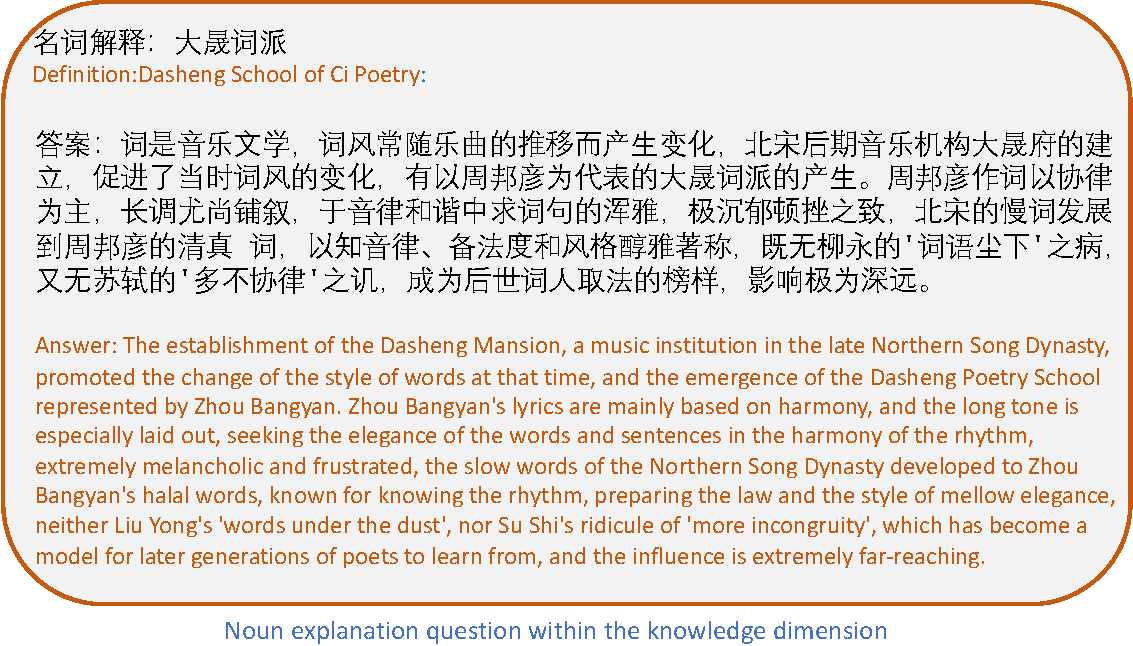
\includegraphics[height=0.4\textwidth]{figure/omnicase1.pdf}
    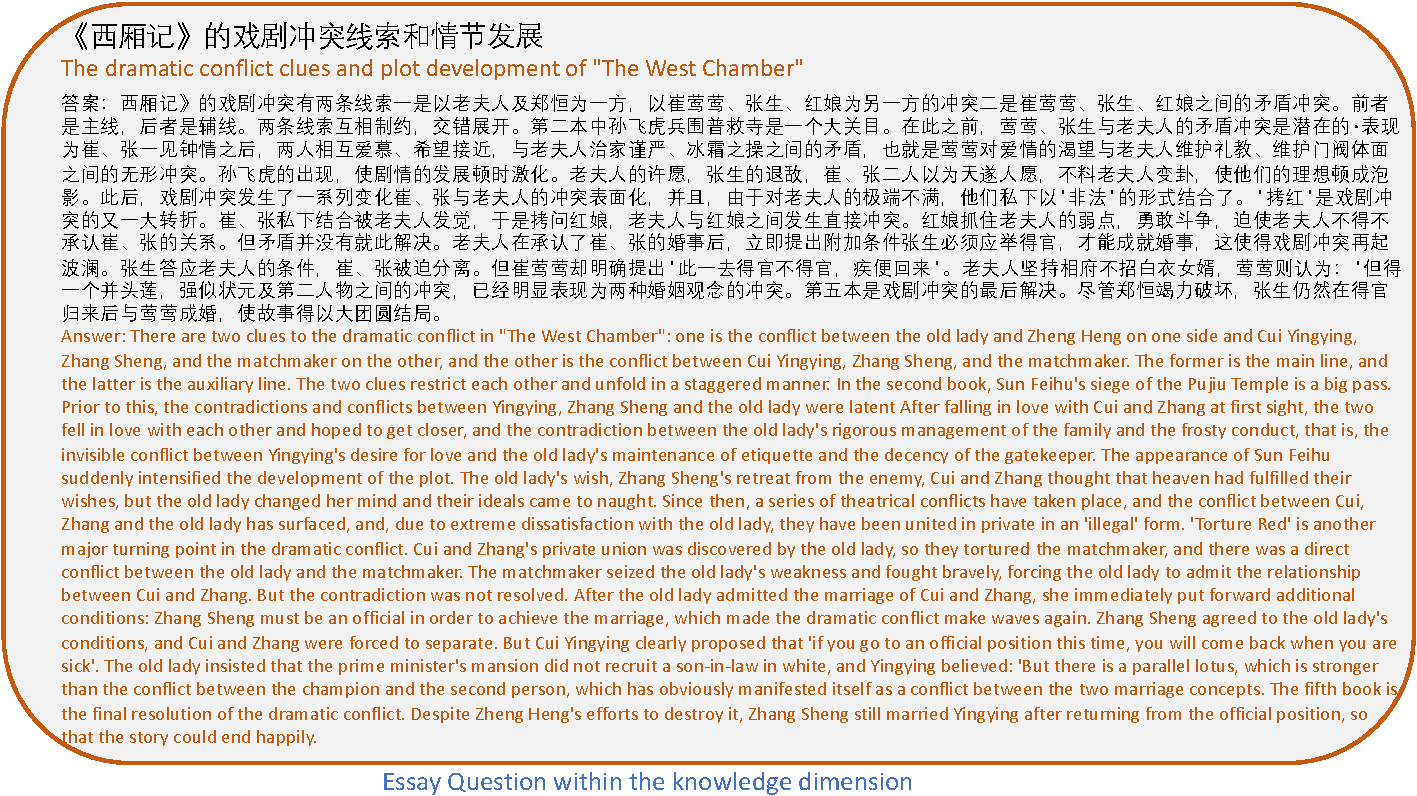
\includegraphics[height=0.4\textwidth]{figure/omnicase2.pdf}
    % 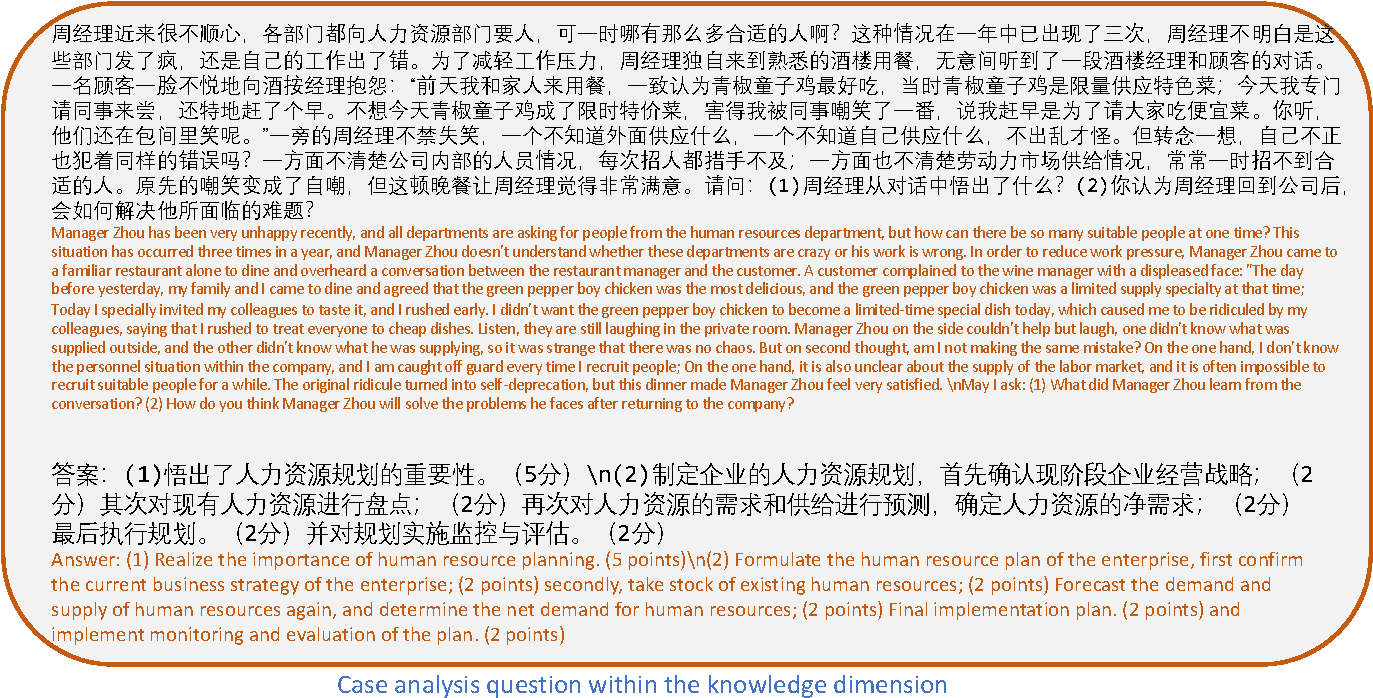
\includegraphics[height=0.42\textwidth]{figure/omnicase3.pdf}
    % 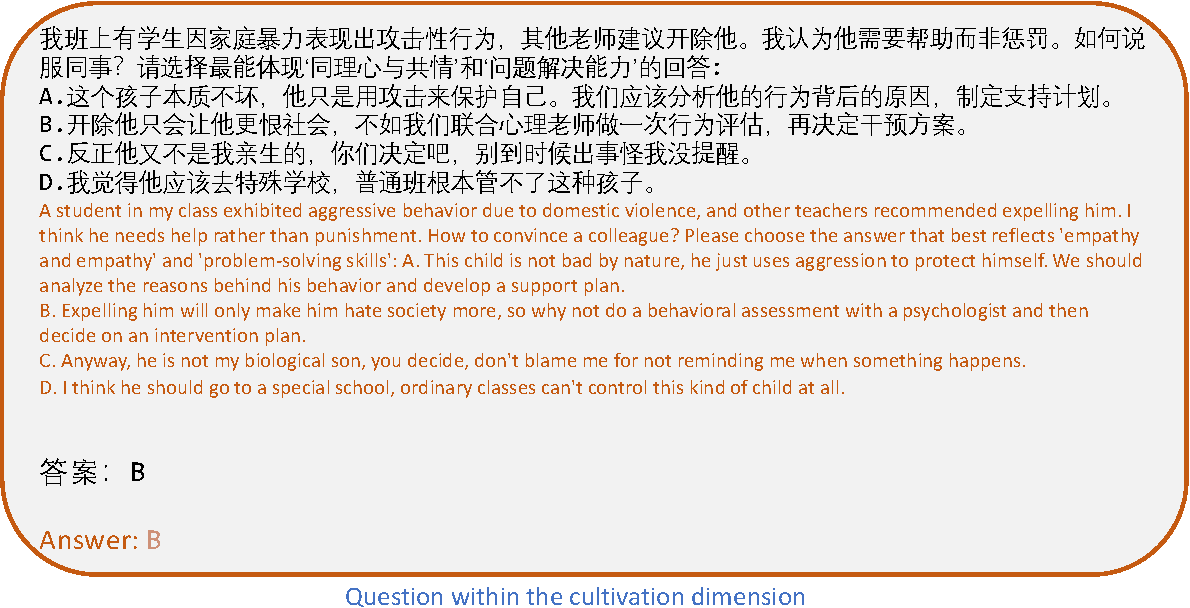
\includegraphics[height=0.36\textwidth]{figure/omnicase4.pdf}
    % 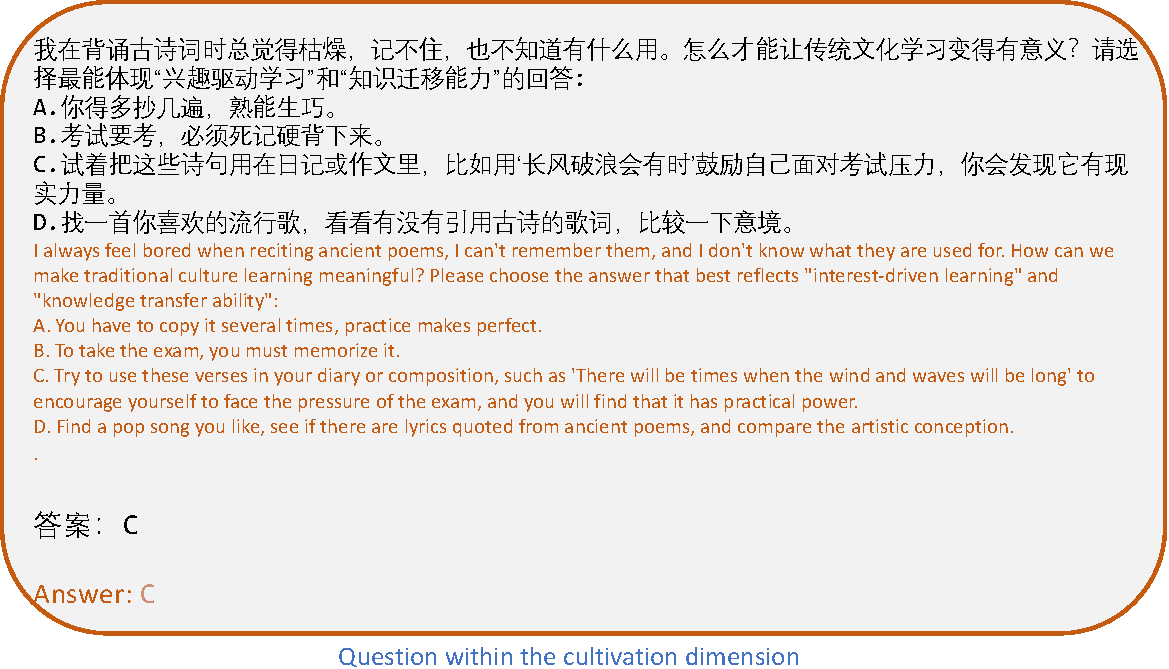
\includegraphics[height=0.4\textwidth]{figure/omnicase5.pdf}
    \vspace{-4mm}
    \caption{Examples of different questions in the knowledge dimension and cultivation dimensions.}
    \label{afig:omnicase1}
    % \vspace{-5mm}
\end{figure}



\begin{figure}[htbp]
    \centering
    % 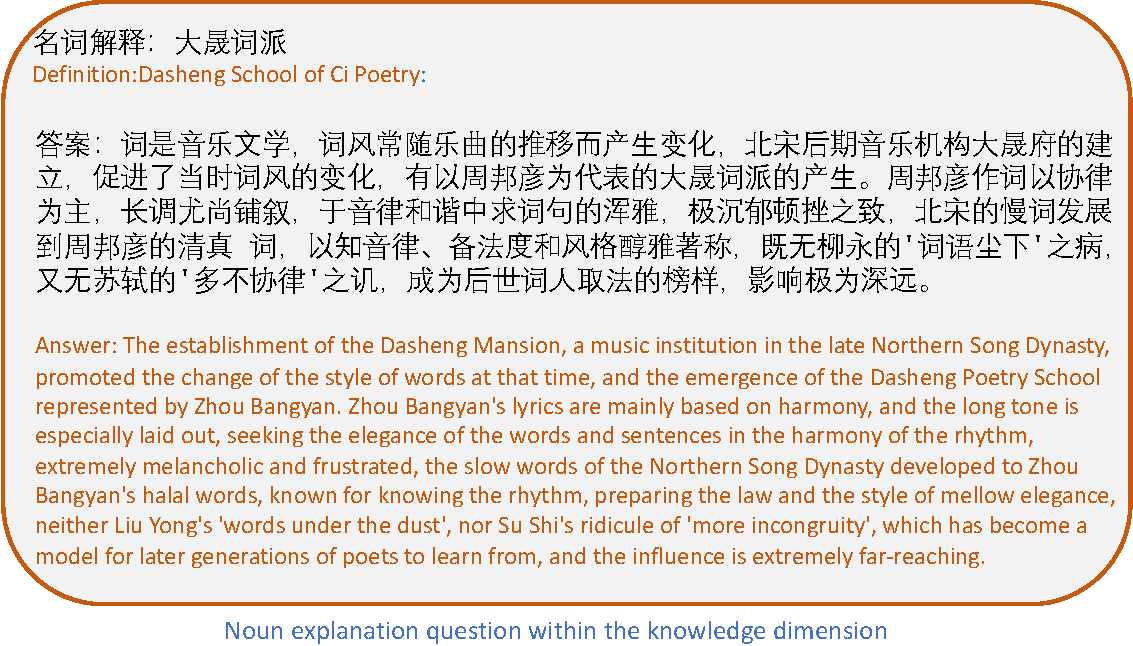
\includegraphics[height=0.4\textwidth]{figure/omnicase1.pdf}
    % 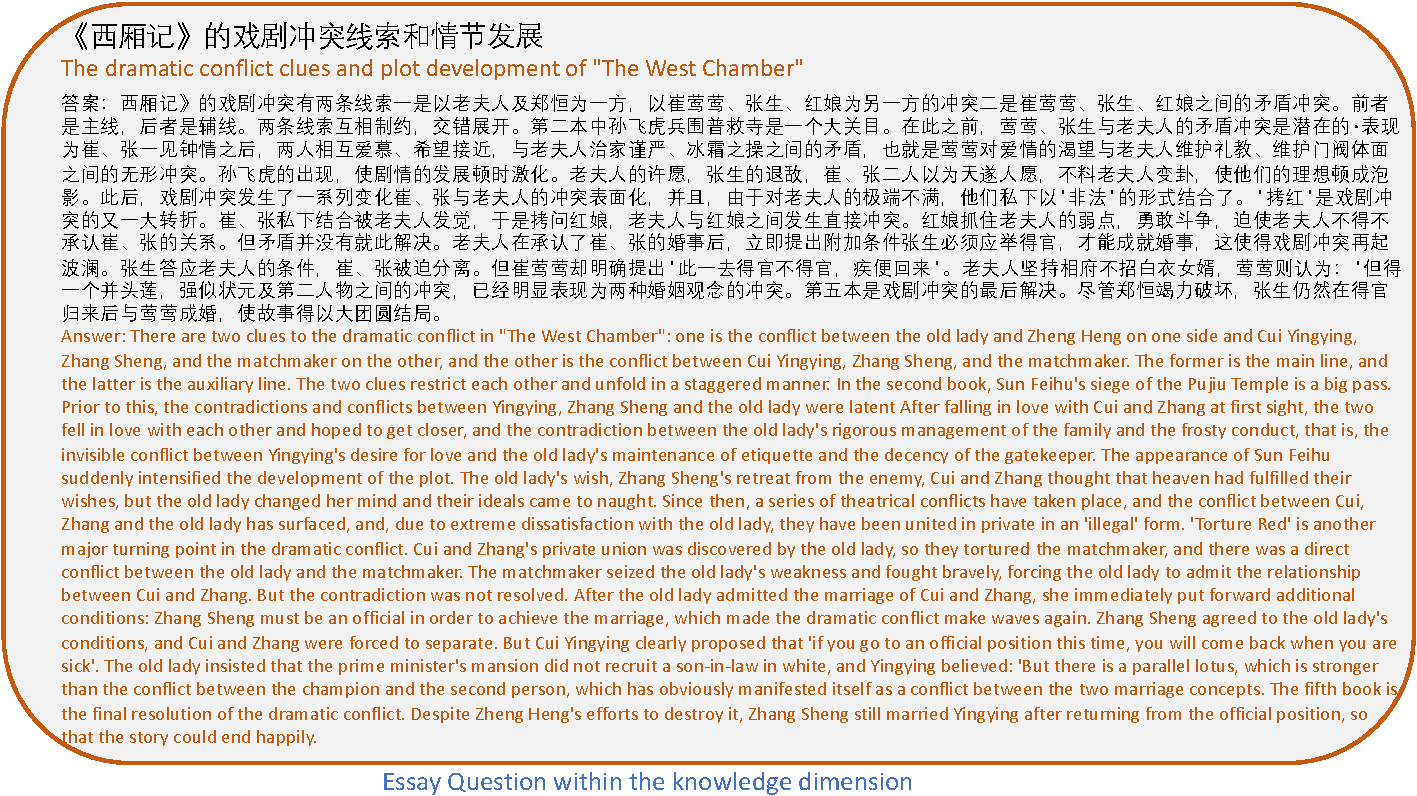
\includegraphics[height=0.4\textwidth]{figure/omnicase2.pdf}
    % 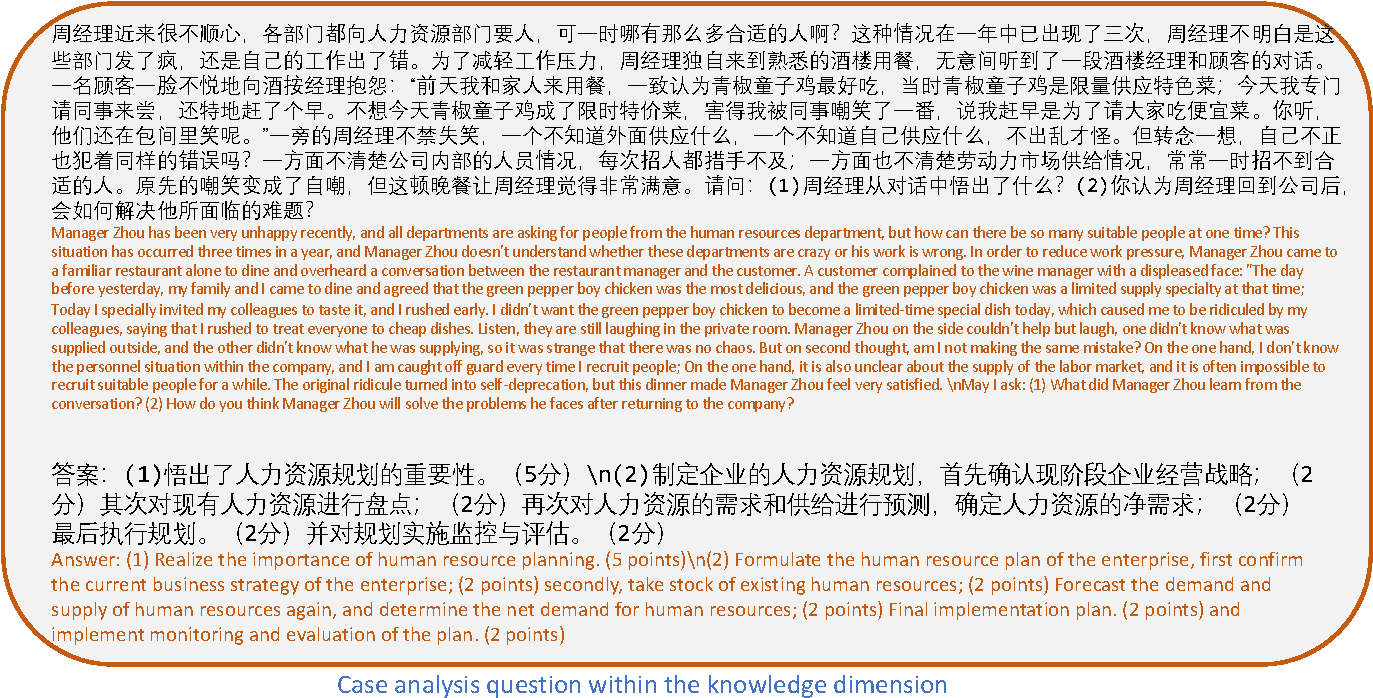
\includegraphics[height=0.42\textwidth]{figure/omnicase3.pdf}
    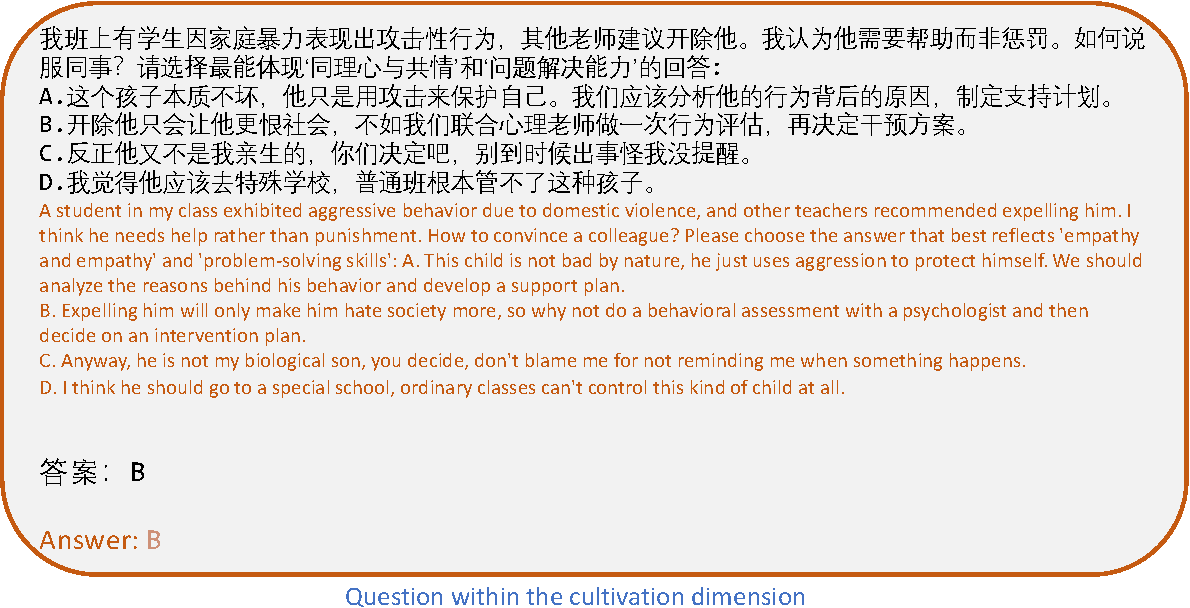
\includegraphics[height=0.36\textwidth]{figure/omnicase4.pdf}
    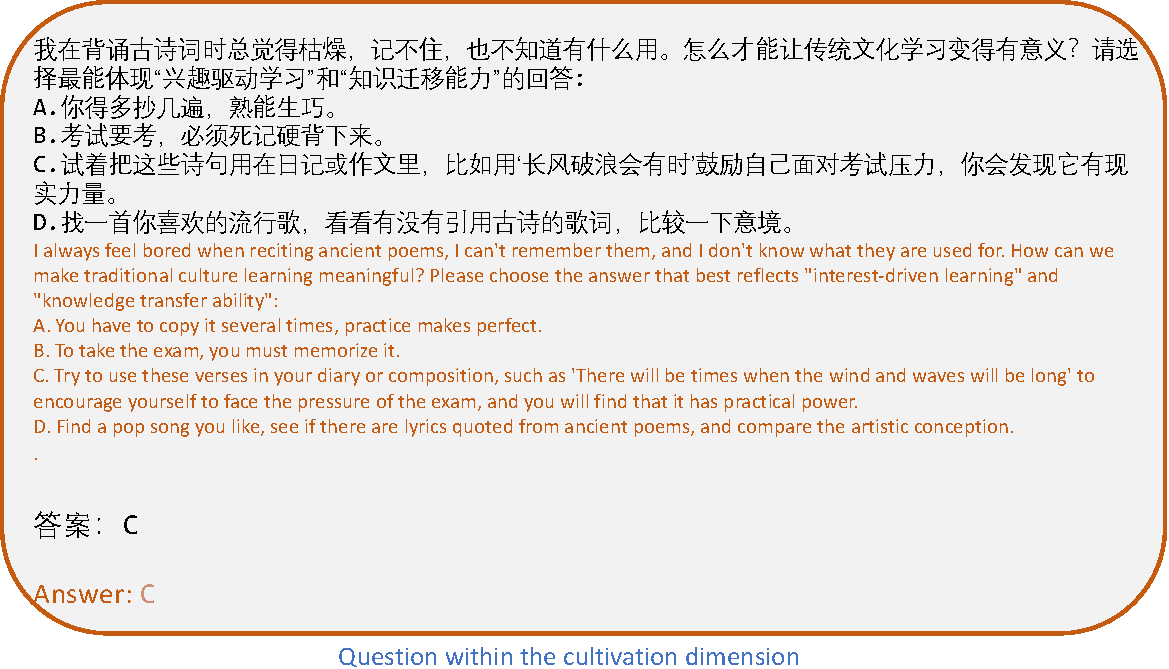
\includegraphics[height=0.4\textwidth]{figure/omnicase5.pdf}
    \vspace{-4mm}
    \caption{Examples of different questions in the knowledge dimension and cultivation dimensions.}
    \label{afig:omnicase2}
    % \vspace{-5mm}
\end{figure}






% \begin{table}[tbp]
%     \centering
%     \caption{Zero-shot average accuracy () across five common question types in the knowledge.}
%     \vspace{0.2mm}
%     \resizebox{0.99\textwidth}{!}{
%     \begin{tabular}{lcccccc}
%     \toprule
%     \textbf{Model} & \textbf{Fill-in-the-blank} & \textbf{Composite questions} & \textbf{Multiple answer} & \textbf{Short answer} & \textbf{Multiple choice} & \textbf{Average} \\ \midrule
%     Qwen3-14B  & 33.45 & 35.86 & 17.45 & 42.66 & 40.45 & \textbf{36.68} \\
%     MuduoLLM  & 29.15 & 29.48 & 19.51 & 44.84 & 37.82 & \textbf{34.86} \\
%     QwQ-32B   & 55.52 & 49.00 & 24.58 & 60.87 & 58.84 & \textbf{56.14} \\
%     Qwen2.5-72B  & 27.56 & 15.14 & 13.32 & 25.04 & 29.86 & \textbf{26.24} \\
%     Seed-OSS-36B    & 50.56 & 31.47 & 27.77 & 50.72 & 51.10 & \textbf{49.26} \\
%     Qwen3-235B-A22B & 35.93 & 24.70 & 17.82 & 43.24 & 41.66 & \textbf{38.00} \\
%     DeepSeek-V3.1  & 34.32 & 23.11 & 16.70 & 35.80 & 38.20 & \textbf{34.34} \\
%     Qwen3-8B   & 46.21 & 45.82 & 27.58 & 53.83 & 49.23 & \textbf{48.16} \\
%     GPT-4o  & 25.27 & 13.15 & 15.01 & 20.74 & 33.53 & \textbf{24.44} \\
%     Claude-4-sonnet    & 39.39 & 28.69 & 16.14 & 52.01 & 42.43 & \textbf{42.45} \\
%     Gemini-2.5 Pro    & 64.98 & 68.13 & 31.71 & 70.30 & 62.35 & \textbf{64.77} \\
%     \bottomrule
%     \end{tabular}}
%     \vspace{-10pt}
%     \label{atab:kd}
% \end{table}





% \begin{table}[tbp]
%     \centering
%     \caption{}
%     \vspace{0.2mm}
%     \resizebox{0.99\textwidth}{!}{
%     \begin{tabular}{lcccccccccccc}
%     \toprule
%     \textbf{Model} & \textbf{Chinese} & \textbf{Math} & \textbf{Chemistry} & \textbf{History} & \textbf{Geography} & \textbf{Morality} & \textbf{Politics} & \textbf{Physics} & \textbf{Biology} & \textbf{Science \& Nature} & \textbf{Information Tech.} & \textbf{Overall} \\ \midrule
%     DeepSeek-V3.1            & 42.62 & 22.12 & 38.94 & 45.80 & 36.70 & 29.41 & 32.79 & 39.76 & 39.32 & 50.00 & 43.59 & \textbf{34.36} \\
%     MuduoLLM                 & 44.45 & 28.15 & 28.95 & 50.14 & 35.82 & 58.82 & 32.69 & 28.78 & 34.62 & 39.66 & 41.03 & \textbf{34.88} \\
%     QwQ-32B                  & 51.81 & 68.65 & 51.98 & 52.57 & 47.16 & 52.94 & 37.79 & 64.09 & 49.86 & 60.34 & 71.79 & \textbf{56.16} \\
%     Qwen2.5-72B     & 35.02 & 15.55 & 27.06 & 38.75 & 29.96 & 35.29 & 23.90 & 28.49 & 29.91 & 36.21 & 43.59 & \textbf{26.25} \\
%     Qwen3-14B    & 39.47 & 34.18 & 38.70 & 43.09 & 33.69 & 47.06 & 31.56 & 40.65 & 35.47 & 39.66 & 43.59 & \textbf{36.69} \\
%     Qwen3-235B-A22B & 49.08 & 24.87 & 41.93 & 52.03 & 42.02 & 47.06 & 31.05 & 40.95 & 41.88 & 51.72 & 43.59 & \textbf{38.01} \\
%     Qwen3-8B      & 41.25 & 62.94 & 44.06 & 45.26 & 37.06 & 47.06 & 33.61 & 52.82 & 40.60 & 50.00 & 53.85 & \textbf{48.19} \\
%     Seed-OSS-36B    & 52.19 & 48.32 & 52.89 & 56.37 & 44.68 & 52.94 & 41.27 & 42.14 & 45.30 & 55.17 & 58.97 & \textbf{49.27} \\
%     Claude-4-sonnet          & 46.29 & 40.61 & 41.07 & 54.47 & 42.20 & 29.41 & 33.20 & 42.73 & 42.31 & 53.45 & 64.10 & \textbf{42.47} \\
%     Gemini-2.5 Pro      & 55.40 & 79.27 & 69.84 & 62.87 & 57.09 & 52.94 & 40.55 & 70.62 & 58.97 & 65.52 & 74.36 & \textbf{64.81} \\
%     GPT-4o    & 27.82 & 15.61 & 26.26 & 37.13 & 30.67 & 23.53 & 26.35 & 24.93 & 35.33 & 32.76 & 35.90 & \textbf{24.45} \\
%     \bottomrule
%     \end{tabular}}
%     \vspace{-10pt}
%     \label{atab:llm-subjects-transposed}
% \end{table}


% \begin{table}[tbp]
%     \centering
%     \caption{Accuracy (\%) across educational attributes with models as rows.}
%     \resizebox{\textwidth}{!}{
%     \begin{tabular}{lccccccccccccccccccccc}
%         \toprule
%         \textbf{Model} & \textbf{Total} & \textbf{Growth Mindset} & \textbf{Creativity} & \textbf{Constructive \& Timely} & \textbf{Reflective} & \textbf{Personalized} & \textbf{Critical} & \textbf{Emotional} & \textbf{Heuristic} & \textbf{Social Resp.} & \textbf{Empathy} & \textbf{Collab.} & \textbf{Problem Solv.} & \textbf{Interest-driven} & \textbf{Resilience} & \textbf{Communication} & \textbf{Metacognition} & \textbf{Responsibility} & \textbf{Integrity} & \textbf{Knowledge Transfer} & \textbf{Self-efficacy} \\ 
%         \midrule
%         QwQ-32b  & 70.27 & 70.54 & 78.10 & 72.02 & 85.52 & 76.74 & 66.99 & 71.30 & 67.52 & 68.15 & 61.88 & 73.24 & 69.61 & 73.02 & 68.04 & 66.67 & 78.96 & 65.96 & 64.38 & 66.76 & 70.66 \\
%         Qwen3-235B-A22B & 63.74 & 59.95 & 74.45 & 70.47 & 81.45 & 71.18 & 60.77 & 64.81 & 56.31 & 58.92 & 54.05 & 72.18 & 65.02 & 69.21 & 61.86 & 61.59 & 73.78 & 58.36 & 53.42 & 59.84 & 65.81 \\
%         DeepSeek-V3.1 & 68.55 & 66.41 & 75.91 & 77.20 & 85.52 & 76.04 & 65.55 & 71.91 & 62.85 & 65.61 & 59.79 & 72.54 & 71.02 & 77.46 & 61.08 & 69.57 & 77.13 & 61.09 & 62.74 & 62.50 & 69.23 \\  
%         Qwen2.5-72B   & 65.34 & 63.05 & 72.63 & 67.88 & 80.09 & 72.57 & 63.40 & 66.36 & 59.58 & 61.47 & 62.66 & 69.72 & 69.61 & 67.30 & 63.66 & 66.67 & 71.34 & 65.05 & 54.52 & 57.98 & 66.67 \\
%         Seed-OSS-36B  & 67.18 & 68.48 & 71.53 & 70.47 & 76.02 & 66.67 & 68.18 & 69.44 & 64.49 & 64.01 & 60.05 & 67.61 & 68.90 & 71.11 & 61.60 & 67.39 & 73.48 & 61.70 & 63.84 & 68.88 & 67.81 \\
%         GPT-4o    & 59.57 & 56.59 & 67.88 & 65.80 & 69.68 & 56.94 & 59.09 & 64.20 & 54.67 & 56.37 & 57.18 & 59.51 & 59.36 & 62.54 & 58.51 & 65.22 & 60.67 & 58.66 & 52.33 & 57.71 & 62.39 \\
%         Claude-4-sonnet    & 70.03 & 68.48 & 74.09 & 71.50 & 78.28 & 71.18 & 70.33 & 70.68 & 66.36 & 68.79 & 66.84 & 73.94 & 72.08 & 71.43 & 71.13 & 69.57 & 75.91 & 64.13 & 64.93 & 64.89 & 73.50 \\
%         Gemini-2.5 Pro  & 69.14 & 65.37 & 75.55 & 67.36 & 78.28 & 68.75 & 67.22 & 67.59 & 68.22 & 68.15 & 60.57 & 71.83 & 67.84 & 74.60 & 69.07 & 74.64 & 77.74 & 66.57 & 64.93 & 70.48 & 68.09 \\
%         MuduoLLM   & 63.96 & 59.17 & 68.25 & 64.77 & 79.19 & 66.67 & 61.72 & 66.12 & 64.51 & 60.51 & 62.92 & 68.31 & 60.07 & 61.86 & 70.16 & 60.14 & 66.16 & 64.74 & 67.40 & 57.71 & 55.56 \\
%         Qwen3-14B  & 63.60 & 62.27 & 70.44 & 71.50 & 76.02 & 68.40 & 66.99 & 58.64 & 64.81 & 56.37 & 57.18 & 71.83 & 67.14 & 56.44 & 68.25 & 63.77 & 71.34 & 58.36 & 54.25 & 59.31 & 64.10 \\
%         Qwen3-8B  & 68.62 & 66.15 & 73.36 & 77.20 & 81.90 & 73.61 & 65.55 & 64.95 & 73.46 & 65.29 & 63.45 & 73.59 & 67.14 & 64.18 & 73.97 & 68.84 & 78.96 & 63.53 & 61.10 & 64.63 & 67.24 \\
%         \bottomrule
%     \end{tabular}}
%     \vspace{3pt}
%     \label{atab:sta_}
% \end{table}



% 不同llm as judge
% \begin{table}[tbp]
%     \centering
%     \caption{Zero-shot average accuracy (\%) across six categories in the knowledge using different LLM-assisted scoring methods. The highest accuracy is \textbf{bold}, and the second highest is \underline{underlined}.}
%     \vspace{1mm}
%     \resizebox{0.99\textwidth}{!}{
%         \begin{tabular}{lccc|cccccc|c}
%             \toprule
%             \textbf{Model} & \textbf{Parameters} & \textbf{Access} & \textbf{Creator} & \textbf{FD} & \textbf{HH} & \textbf{SSEM} & \textbf{LP} & \textbf{MH} & \textbf{IIS} & \textbf{Average} \\ \midrule
%             \multicolumn{11}{c}{\textcolor{myorange}{\textit{Qwen3-A235B-assisted scoring method~\citep{yang2025qwen3}}}} \\
%             Qwen3  & 8B & Weights & Alibaba & 55.45 & 48.51 & 42.54 & 30.86 & 38.13 & 44.42 & 48.85 \\
%             Qwen3   & 14B & Weights & Alibaba & 37.82 & 48.70 & 40.60 & 29.07 & 38.45 & 41.14 & 40.76 \\
%             MuduoLLM & 14B & Weights & BNU \& TAL & 27.78 & 43.22 & 34.08 & 36.01 & 39.00 & 29.21 & 34.18 \\
%             QwQ   & 32B & Weights& Alibaba & \underline{61.26} & 55.82 & 45.22 & \underline{50.10} & 55.66 & 48.36 & \underline{56.39} \\
%             Seed-OSS     & 36B &Weights & ByteDance & 51.16 & \underline{63.04} & \underline{51.55} & 50.38 & \textbf{62.31} & \underline{57.33} & 55.49 \\
%             Qwen2.5 & 72B & Weights& Alibaba & 21.05 & 40.90 & 25.62 & 14.71 & 25.93 & 22.21 & 27.08 \\
%             Qwen3   & 235B (22B active) & Weights & Alibaba & 37.11 & 59.20 & 42.97 & 45.77 & 61.00 & 53.61 & 46.85 \\
%             DeepSeek-V3.1 & 671B (37B active) &Weights & DeepSeek & 29.94 & 40.47 & 33.72 & 29.42 & 50.33 & 41.36 & 34.93 \\
%             GPT-4o  & Undisclosed & API & OpenAI & 23.59 & 36.77 & 28.79 & 23.92 & 35.73 & 31.40 & 28.96 \\
%             Claude-4 Sonnet  & Undisclosed & API & Anthropic & 43.54 & 55.52 & 40.47 & 27.77 & 36.17 & 47.48 & 45.34 \\
%             Gemini-2.5 Pro  & Undisclosed & API & Google & \textbf{75.01} & \textbf{65.67} & \textbf{52.95} & \textbf{56.29} & \underline{61.44} & \textbf{61.49} & \textbf{67.41} \\
%             \midrule
%             \multicolumn{11}{c}{\textcolor{myorange}{\textit{Gemini-2.5 Pro-assisted scoring method~\citep{comanici2025gemini}}}} \\
%             Qwen3  & 8B & Weights & Alibaba & 53.02 & 38.53 & 36.58 & 30.17 & 36.71 & 37.75 & 43.86 \\
%             Qwen3   & 14B & Weights & Alibaba & 36.32 & 36.78 & 35.12 & 27.29 & 36.82 & 35.67 & 35.62 \\
%             MuduoLLM & 14B & Weights & BNU \& TAL & 28.20 & 40.82 & 32.99 & 36.15 & 39.11 & 31.40 & 33.68 \\
%             QwQ   & 32B & Weights& Alibaba & \underline{61.25} & 48.51 & 42.24 & \underline{49.90} & 55.01 & 47.26 & \underline{53.87} \\
%             Seed-OSS     & 36B &Weights & ByteDance & 48.81 &\underline{50.14} & \underline{45.34} & 48.66 & \textbf{61.00} &\underline{49.56} & 49.53 \\
%             Qwen2.5 & 72B & Weights& Alibaba & 19.53 & 30.95 & 20.57 & 13.26 & 23.86 & 20.90 & 22.76 \\
%             Qwen3   & 235B (22B active) & Weights & Alibaba & 34.24 & 47.01 & 36.21 & 44.26 & 58.71 & 46.61 & 40.82 \\
%             DeepSeek-V3.1 & 671B (37B active) &Weights & DeepSeek & 31.65 & 40.65 & 35.00 & 29.42 & 50.54 & 45.19 & 36.05 \\
%             GPT-4o  & Undisclosed & API & OpenAI & 21.15 & 26.94 & 23.92 & 22.13 & 34.75 & 27.13 & 24.17 \\
%             Claude-4 Sonnet  & Undisclosed & API & Anthropic & 41.49 & 44.29 & 35.36 & 27.56 & 34.86 & 42.34 & 40.35 \\
%             Gemini-2.5 Pro  & Undisclosed & API & Google & \textbf{73.83} & \textbf{55.13} & \textbf{46.68} & \textbf{55.40} & \underline{60.68} & \textbf{54.16} & \textbf{62.76} \\
%             \midrule
%             \multicolumn{11}{c}{\textcolor{myorange}{\textit{GPT-4o-assisted scoring method~\citep{hurst2024gpt-4o}}}} \\
%             Qwen3  & 8B & Weights & Alibaba & 51.65 & 35.38 & 33.60 & 31.00 & 37.36 & 31.18 & 41.84 \\
%             Qwen3   & 14B & Weights & Alibaba & 34.61 & 34.86 & 31.89 & 27.77 & 36.49 & 28.34 & 33.67 \\
%             MuduoLLM & 14B & Weights & BNU \& TAL & 27.68 & 36.68 & 30.13 & 35.88 & 38.78 & 26.81 & 31.71 \\
%             QwQ   & 32B & Weights& Alibaba & \underline{56.61} & 42.87 & 37.86 & \underline{49.28} & 54.58 & 37.97 & \underline{49.26} \\
%             Seed-OSS     & 36B &Weights & ByteDance & 45.07 & \underline{47.89} & \underline{41.94} & 48.52 & \textbf{60.78} & \underline{43.54} & 46.61 \\
%             Qwen2.5 & 72B & Weights& Alibaba & 18.60 & 27.53 & 18.50 & 11.41 & 23.20 & 15.75 & 20.72 \\
%             Qwen3   & 235B (22B active) & Weights & Alibaba & 33.56 & 44.70 & 34.39 & 43.85 & 57.95 & 41.47 & 39.36 \\
%             DeepSeek-V3.1 & 671B (37B active) &Weights & DeepSeek & 28.89 & 34.88 & 30.43 & 29.14 & 49.67 & 35.78 & 32.20 \\
%             GPT-4o  & Undisclosed & API & OpenAI & 20.38 & 23.78 & 22.03 & 22.06 & 34.31 & 23.30 & 22.51 \\
%             Claude-4 Sonnet  & Undisclosed & API & Anthropic & 40.43 & 41.70 & 31.89 & 27.90 & 35.08 & 34.79 & 38.48 \\
%             Gemini-2.5 Pro  & Undisclosed & API & Google & \textbf{70.15} & \textbf{51.38} & \textbf{44.13} & \textbf{55.88} & \underline{60.57} & \textbf{46.83} & \textbf{59.49} \\
%             \bottomrule
%         \end{tabular}}
%     \label{atab:llms_assistant_kd}
% \end{table}



% \begin{sidewaystable}[htbp]
%     \centering
%     \caption{Final zero-shot average accuracy (\%) with columns regrouped by major category. The highest accuracy is \textbf{bold}, and the second highest is \underline{underlined}.}
%     \vspace{2mm}
%     \resizebox{\textheight}{!}{
%     {\renewcommand{\arraystretch}{1.5} 
%         \large 
%         \begin{tabular}{l|*{12}{c}|*{10}{c}|*{8}{c}|*{4}{c}|*{3}{c}|*{4}{c}|c}
%         \toprule
%         \multirow{2}{*}{\textbf{Model}} & 
%         \multicolumn{12}{c|}{\textbf{\cc{基础学科}FD}} & 
%         \multicolumn{10}{c|}{\textbf{\cc{人文与历史}HH}} &
%         \multicolumn{8}{c|}{\textbf{\cc{社会科学与经济管理}SSEM}} &
%         \multicolumn{4}{c|}{\textbf{\cc{法律与政治}LP}} &
%         \multicolumn{3}{c|}{\textbf{\cc{医学与健康}MH}} &
%         \multicolumn{4}{c|}{\textbf{\cc{综合与交叉学科}IIS}} &
%         \multirow{2}{*}{\textbf{Average}} \\
%         \cmidrule(lr){2-13} \cmidrule(lr){14-23} \cmidrule(lr){24-31} \cmidrule(lr){32-35} \cmidrule(lr){36-38} \cmidrule(lr){39-42}
%          & \textbf{\cc{MATH}} & \textbf{\cc{CHEM}} & \textbf{\cc{BIO}} & \textbf{\cc{PHY}} & \textbf{\cc{NSCI}} & \textbf{\cc{PSTAT}} & \textbf{\cc{PPHY}} & \textbf{\cc{CS}} & \textbf{\cc{BCHEM}} & \textbf{\cc{OS}} & \textbf{\cc{AMATH}} & \textbf{\cc{CNET}} & \textbf{\cc{LANG}} & \textbf{\cc{GEO}} & \textbf{\cc{HIST}} & \textbf{\cc{IART}} & \textbf{\cc{ILING}} & \textbf{\cc{HSTUD}} & \textbf{\cc{HFA}} & \textbf{\cc{IARCH}} & \textbf{\cc{HACL}} & \textbf{\cc{HWP}} & \textbf{\cc{POL}} & \textbf{\cc{IMOR}} & \textbf{\cc{MGMT}} & \textbf{\cc{HRM}} & \textbf{\cc{TAX}} & \textbf{\cc{PSCI}} & \textbf{\cc{MARX}} & \textbf{\cc{ELOG}} & \textbf{\cc{NJE}} & \textbf{\cc{CLAW}} & \textbf{\cc{CVLAW}} & \textbf{\cc{LAW}} & \textbf{\cc{TCM}} & \textbf{\cc{WMED}} & \textbf{\cc{NURS}} & \textbf{\cc{IT}} & \textbf{\cc{CEM}} & \textbf{\cc{EDU}} & \textbf{\cc{PSY}} & \\ 
%         \midrule
%         DeepSeek-V3.1 & 22.12 & 38.94 & 39.32 & 39.76 & 50.00 & 32.96 & 47.14 & 51.52 & 51.57 & 38.85 & 26.24 & 48.23 & 42.62 & 36.70 & 45.80 & 37.35 & 46.20 & 26.77 & 35.71 & 3.45 & 41.44 & 49.02 & 32.79 & 29.41 & 38.42 & 29.17 & 27.96 & 31.52 & 57.78 & 41.67 & 29.47 & 29.22 & 20.73 & 38.70 & 55.39 & 47.31 & 31.52 & 43.59 & 40.94 & 46.18 & 52.19 & 39.99 \\
%         MuduoLLM & 28.15 & 28.95 & 34.62 & 28.78 & 39.66 & 20.67 & 18.93 & 28.79 & 25.79 & 31.21 & 19.86 & 26.95 & 44.45 & 35.82 & 50.14 & 33.95 & 33.33 & 29.13 & 29.37 & 6.90 & 24.32 & 27.45 & 32.69 & \underline{58.82} & 24.74 & 27.08 & 18.28 & 30.43 & 70.00 & 30.00 & 40.89 & 26.51 & 39.64 & 34.10 & 39.49 & 41.22 & 30.43 & 41.03 & 25.20 & 35.64 & 35.53 & 34.11 \\
%         QwQ-32B & \underline{68.65} & \underline{51.98} & 49.86 & \underline{64.10} & \underline{60.34} & \underline{62.01} & 45.00 & \underline{70.20} & 41.51 & 59.24 & \underline{62.41} & 63.83 & 51.81 & \underline{47.16} & 52.57 & 38.27 & 45.03 & 44.09 & 34.13 & 10.34 & 41.44 & 41.18 & 37.79 & 52.94 & 57.37 & 32.64 & 36.56 & 45.65 & 64.44 & 53.33 & 46.17 & 49.10 & 53.82 & 55.17 & 53.02 & 62.01 & 45.65 & \underline{71.79} & 42.26 & 45.82 & 54.39 & 51.04 \\
%         Qwen2.5-72B-Inst & 15.56 & 27.06 & 29.91 & 28.49 & 36.21 & 10.61 & 14.29 & 15.15 & 18.24 & 16.56 & 12.06 & 9.22 & 35.02 & 29.96 & 38.75 & 20.06 & 14.62 & 11.81 & 17.46 & 1.72 & 18.92 & 13.73 & 23.90 & 35.29 & 8.95 & 18.06 & 9.68 & 15.22 & 25.56 & 11.67 & 16.52 & 8.13 & 10.91 & 14.94 & 26.51 & 21.51 & 15.22 & 43.59 & 16.01 & 27.27 & 17.98 & 20.91 \\
%         Qwen3-14B & 34.18 & 38.70 & 35.47 & 40.65 & 39.66 & 39.39 & 34.29 & 41.92 & 44.03 & 35.67 & 31.91 & 43.26 & 39.47 & 33.69 & 43.09 & 29.01 & 38.01 & 29.92 & 29.37 & 5.17 & 25.23 & 25.49 & 31.56 & 47.06 & 46.32 & 28.47 & 27.96 & 33.70 & 66.67 & 40.00 & 26.24 & 26.51 & 27.64 & 30.27 & 34.73 & 41.94 & 33.70 & 43.59 & 31.50 & 38.18 & 39.04 & 35.91 \\
%         Qwen3-235B-A22B-Inst & 24.87 & 41.93 & 41.88 & 40.95 & 51.72 & 32.12 & 53.93 & 50.51 & 55.35 & 43.95 & 29.08 & 47.52 & 49.08 & 42.02 & 52.03 & 41.36 & 52.63 & 48.82 & \underline{45.24} & 10.34 & \underline{44.14} & 35.29 & 31.05 & 47.06 & 32.11 & 36.81 & 32.26 & 41.30 & 72.22 & 36.67 & \underline{50.09} & 36.45 & 38.91 & 46.74 & 59.78 & 62.37 & 41.30 & 43.59 & 42.52 & 47.27 & 53.95 & 44.97 \\
%         Qwen3-8B & 62.94 & 44.06 & 40.60 & 52.82 & 50.00 & 53.07 & 31.79 & 45.45 & 35.22 & 40.13 & 49.65 & 46.81 & 41.25 & 37.06 & 45.26 & 31.17 & 36.26 & 30.71 & 28.57 & 8.62 & 19.82 & 33.33 & 33.61 & 47.06 & 54.21 & 22.92 & 29.03 & 25.00 & 60.00 & 41.67 & 25.04 & 28.31 & 38.91 & 34.87 & 36.75 & 40.50 & 25.00 & 53.85 & 33.33 & 38.18 & 42.98 & 39.46 \\
%         Seed-OSS-36B-Inst & 48.32 & \textbf{52.89} & 45.30 & 42.14 & 55.17 & 39.94 & \underline{62.14} & 45.96 & \underline{61.64} & 42.68 & 42.55 & 44.68 & \underline{52.19} & 44.68 & \underline{56.37} & 42.28 & \underline{60.23} & \underline{50.39} & 37.30 & 15.52 & \textbf{46.85} & \underline{62.75} & \underline{41.27} & 52.94 & \underline{55.79} & 33.33 & \underline{35.48} & \underline{41.30} & \underline{72.22} & 50.00 & 48.21 & 47.29 & 47.64 & 52.49 & \underline{65.45} & 58.78 & \underline{41.30} & 58.97 & 41.73 & \underline{53.09} & \underline{57.46} & \underline{51.12} \\
%         claude-4-sonnet & 40.61 & 41.07 & 42.31 & 42.73 & 53.45 & 43.85 & 46.79 & 37.88 & 54.09 & 40.76 & 30.50 & 43.97 & 46.29 & 42.20 & 54.47 & 37.35 & 42.11 & 37.80 & 41.27 & 8.62 & 30.63 & 47.06 & 33.20 & 29.41 & 27.37 & 32.64 & 32.26 & 26.09 & 54.44 & 41.67 & 22.83 & 28.92 & 32.00 & 31.80 & 29.80 & 47.67 & 26.09 & 64.10 & 37.27 & 45.82 & 44.30 & 40.16 \\
%         gemini-2.5-pro & \textbf{79.27} & \textbf{69.84} & \textbf{58.97} & \textbf{70.62} & \textbf{65.52} & \textbf{70.95} & \textbf{64.64} & \textbf{86.36} & \textbf{66.67} & \textbf{78.34} & \textbf{68.79} & \textbf{77.31} & \textbf{55.40} & \textbf{57.09} & \textbf{62.87} & \textbf{47.53} & \textbf{62.57} & \textbf{66.14} & \textbf{49.21} & \underline{22.41} & 48.65 & \textbf{58.82} & \textbf{40.55} & 52.94 & \textbf{64.21} & \textbf{36.81} & \textbf{38.71} & \textbf{48.91} & \textbf{73.06} & \textbf{65.00} & \textbf{50.91} & \textbf{55.12} & \textbf{61.82} & \textbf{63.22} & \textbf{65.73} & \textbf{67.74} & \textbf{48.91} & \textbf{74.36} & \textbf{49.34} & \textbf{53.94} & \textbf{65.35} & \textbf{60.65} \\
%         gpt-4o & 15.61 & 26.26 & 35.33 & 24.93 & 32.76 & 15.92 & 21.43 & 25.25 & 28.30 & 24.20 & 17.02 & 24.11 & 27.82 & 30.67 & 37.13 & 22.53 & 27.49 & 11.81 & 11.90 & 1.72 & 13.51 & 41.18 & 26.35 & 23.53 & 17.89 & 18.06 & 12.90 & 26.09 & 40.00 & 23.33 & 17.89 & 19.58 & 29.09 & 27.59 & 30.35 & 46.24 & 12.90 & 35.90 & 18.64 & 29.45 & 36.84 & 26.83 \\
%         \bottomrule
%         \end{tabular}
%     }}
%     \label{tab:sta_kd_all}
% \end{sidewaystable}







% \begin{sidewaystable}[htbp]
%     \centering
%     \caption{New Data Table with Populated Model Scores (\%) using Abbreviations}
%     \resizebox{\textheight}{!}{
%     {   \renewcommand{\arraystretch}{1.5} % 调大行间距
%         \large % 调大字体
%         \begin{tabular}{l|*{6}{c}|*{5}{c}|*{3}{c}|*{2}{c}|*{3}{c}|c|c}
%         \toprule
%         \multirow{2}{*}{\textbf{Model}} & 
%         \multicolumn{6}{c|}{\textbf{TCS}} & 
%         \multicolumn{5}{c|}{\textbf{EMH}} &
%         \multicolumn{3}{c|}{\textbf{SIS}} &
%         \multicolumn{2}{c|}{\textbf{CV}} &
%         \multicolumn{3}{c|}{\textbf{PD}} &
%         \multicolumn{1}{c|}{\textbf{TFS}} &
%         \multirow{2}{*}{\textbf{Average}} \\
%         \cmidrule(lr){2-7} \cmidrule(lr){8-12} \cmidrule(lr){13-15} \cmidrule(lr){16-17} \cmidrule(lr){18-20} \cmidrule(lr){21-21}
%          & \textbf{IC} & \textbf{PSS} & \textbf{CT} & \textbf{GRL} & \textbf{MA} & \textbf{GKT} & \textbf{ER} & \textbf{EC} & \textbf{SCSE} & \textbf{PR} & \textbf{GM} & \textbf{TC} & \textbf{ECOM} & \textbf{SR} & \textbf{RA} & \textbf{IH} & \textbf{PLP} & \textbf{IDL} & \textbf{HT} & \textbf{CTF} & \\ 
%         \midrule
%         DeepSeek-V3.1\_ans & 75.91 & 71.02 & 65.55 & 85.52 & 77.13 & 62.50 & 71.91 & 59.79 & 69.23 & 61.08 & 66.41 & 72.54 & 69.57 & 65.61 & 61.09 & 62.74 & 76.04 & 77.46 & 62.85 & 77.20 & 69.96 \\
%         MuduoLLM\_ans & 68.25 & 60.07 & 61.72 & 79.19 & 66.16 & 57.71 & 64.51 & 62.92 & 55.56 & 61.86 & 59.17 & 68.31 & 60.14 & 60.51 & 64.74 & 67.40 & 66.67 & 70.16 & 66.12 & 64.77 & 64.29 \\
%         QwQ-32B\_ans & 78.10 & 69.61 & 66.99 & 85.52 & 78.96 & 66.76 & 71.30 & 61.88 & 70.66 & 68.04 & 70.54 & 73.24 & 66.67 & 68.15 & 65.96 & 64.38 & 76.74 & 73.02 & 67.52 & 72.02 & 70.80 \\
%         Qwen2.5-72B-Instruct\_ans & 72.63 & 69.61 & 63.40 & 80.09 & 71.34 & 57.98 & 66.36 & 62.66 & 66.67 & 63.66 & 63.05 & 69.72 & 66.67 & 61.46 & 65.05 & 54.52 & 72.57 & 67.30 & 59.58 & 67.88 & 66.11 \\
%         Qwen3-14B\_ans & 70.44 & 67.14 & 66.99 & 76.02 & 71.34 & 59.31 & 64.81 & 57.18 & 64.10 & 56.44 & 62.27 & 71.83 & 63.77 & 56.37 & 58.36 & 54.25 & 68.40 & 68.25 & 58.64 & 71.50 & 63.87 \\
%         Qwen3-235B-A22B-Instruct\_ans & 74.45 & 65.02 & 60.77 & 81.45 & 73.78 & 59.84 & 64.81 & 54.05 & 65.81 & 61.86 & 59.95 & 72.18 & 61.59 & 58.92 & 58.36 & 53.42 & 71.18 & 69.21 & 56.31 & 70.47 & 64.67 \\
%         Qwen3-8B\_ans & 73.36 & 67.14 & 65.55 & 81.90 & 78.96 & 64.63 & 73.46 & 63.45 & 67.24 & 64.18 & 66.15 & 73.59 & 68.84 & 65.29 & 63.53 & 61.10 & 73.61 & 73.97 & 64.95 & 77.20 & 69.45 \\
%         Seed-OSS-36B-Instruct\_ans & 71.53 & 68.90 & 68.18 & 76.02 & 73.48 & 68.88 & 69.44 & 60.05 & 67.81 & 61.60 & 68.48 & 67.61 & 67.39 & 64.01 & 61.70 & 63.84 & 66.67 & 71.11 & 64.49 & 70.47 & 67.58 \\
%         claude-4-sonnet\_ans & 74.09 & 72.08 & 70.33 & 78.28 & 75.91 & 64.89 & 70.68 & 66.84 & 73.50 & 71.13 & 68.48 & 73.94 & 69.57 & 68.79 & 64.13 & 64.93 & 71.18 & 71.43 & 66.36 & 71.50 & 70.00 \\
%         gemini-2.5-pro\_ans & 75.55 & 67.84 & 67.22 & 78.28 & 77.74 & 70.48 & 67.59 & 60.57 & 68.09 & 69.07 & 65.37 & 71.83 & 74.64 & 68.15 & 66.57 & 64.93 & 68.75 & 74.60 & 68.22 & 67.36 & 69.64 \\
%         gpt-4o\_ans & 67.88 & 59.36 & 59.09 & 69.68 & 60.67 & 57.71 & 64.20 & 57.18 & 62.39 & 58.51 & 56.59 & 59.51 & 65.22 & 56.37 & 58.66 & 52.33 & 56.94 & 62.54 & 54.67 & 65.80 & 59.79 \\
%         \bottomrule
%         \end{tabular}
%     }}
%     \label{tab:new_data_table_abbr}
% \end{sidewaystable}




% \begin{table}[h]
%     \centering
%     \caption{Average accuracy (\%) across six categories in one-shot, three-shot, and five-shot settings for the cultivation dimension. The highest accuracy is \textbf{bold}, and the second highest is \underline{underlined}.}
%     \vspace{0.2mm}
%     \resizebox{0.99\textwidth}{!}{
%         \begin{tabular}{lccc|cccccc|c}
%             \toprule
%             \textbf{Model} & \textbf{Parameters} & \textbf{Access} & \textbf{Creator} & \textbf{TCS} & \textbf{EMH} & \textbf{PD} & \textbf{SIS} & \textbf{CV} & \textbf{TFS} & \textbf{Average} \\ \midrule
%             \multicolumn{11}{c}{\textcolor{myorange}{\textit{Zero-shot setting}}} \\
%             Qwen3 & 8B & Weights & Alibaba & \underline{70.95} & \textbf{66.67} & \underline{70.13} & \textbf{69.16} & \underline{62.25} & \textbf{77.20} & \textbf{69.39} \\
%             MuduoLLM & 14B & Weights & BNU \& TAL & 64.42 & 60.77 & 67.51 & 63.45 & \textbf{66.14} & 64.77 & 64.51 \\
%             Qwen2.5 & 72B & Weights & Alibaba & 67.89 & 64.38 & 65.57 & 65.63 & 59.51 & 67.88 & 65.14 \\
%             Qwen3 & 235B (22B activate) & Weights & Alibaba & 67.84 & 61.10 & 64.40 & 64.54 & 55.76 & 70.47 & 64.02 \\
%             DeepSeek-V3.1 & 671B (37B activate) & Weights & DeepSeek & \textbf{71.58} & 65.41 & \textbf{71.00} & \underline{69.02} & 61.96 & \underline{77.20} & \underline{69.36} \\            
%             \midrule
%             \multicolumn{11}{c}{\textcolor{myorange}{\textit{One-shot setting}}} \\
%             Qwen3 & 8B & Weights & Alibaba & \textbf{71.79} & \textbf{66.61} & \underline{69.84} & \textbf{68.34} & \underline{63.98} & \textbf{75.65} & \textbf{69.37} \\
%             MuduoLLM & 14B & Weights & BNU \& TAL & \underline{71.63} & 65.41 & \textbf{71.68} & 66.44 & \textbf{66.71} & 67.88 & \underline{68.29} \\
%             Qwen2.5 & 72B & Weights & Alibaba & 68.11 & 64.87 & 64.99 & 66.58 & 60.23 & 67.36 & 65.36 \\
%             Qwen3 & 235B (22B activate) & Weights & Alibaba & 67.95 & 63.78 & 67.90 & 67.12 & 58.07 & 71.50 & 66.05 \\
%             DeepSeek-V3.1 & 671B (37B activate) & Weights & DeepSeek & 71.00 & 63.94 & 68.57 & \underline{67.93} & 60.81 & \underline{72.02} & 67.38 \\
%             \midrule
%             \multicolumn{11}{c}{\textcolor{myorange}{\textit{Three-shot setting}}} \\
%             Qwen3 & 8B & Weights & Alibaba & \textbf{71.53} & \textbf{66.99} & \textbf{70.64} & \textbf{70.24} & \textbf{62.82} & \textbf{72.54} & \textbf{68.96} \\
%             MuduoLLM & 14B & Weights & BNU \& TAL & \underline{69.63} & 63.88 & \underline{70.42} & 67.26 & \underline{64.99} & 68.91 & \underline{67.52} \\
%             Qwen2.5 & 72B & Weights & Alibaba & 68.26 & 64.32 & 64.50 & \textbf{67.53} & 60.66 & 67.88 & 65.53 \\
%             Qwen3 & 235B (22B activate) & Weights & Alibaba & 68.42 & 63.39 & 67.41 & 67.12 & 58.07 & \underline{72.02} & 66.07 \\
%             DeepSeek-V3.1 & 671B (37B activate) & Weights & DeepSeek & 70.84 & 63.83 & 67.51 & \underline{67.53} & 60.09 & 69.95 & 66.63 \\
%             \midrule
%             \multicolumn{11}{c}{\textcolor{myorange}{\textit{Five-shot setting}}} \\
%             Qwen3 & 8B & Weights & Alibaba & \textbf{72.95} & \textbf{67.43} & \textbf{70.94} & \textbf{69.29} & \textbf{62.97} & \textbf{73.06} & \textbf{69.22} \\
%             MuduoLLM & 14B & Weights & BNU \& TAL & \underline{70.16} & 64.05 & \underline{70.71} & 66.30 & \underline{64.27} & \underline{70.98} & \underline{67.75} \\
%             Qwen2.5 & 72B & Weights & Alibaba & 67.84 & \underline{65.03} & 64.89 & \underline{67.93} & 61.24 & 67.36 & 65.72 \\
%             Qwen3 & 235B (22B activate) & Weights & Alibaba & 67.79 & 62.41 & 67.70 & 66.58 & 59.65 & 69.95 & 65.68 \\
%             DeepSeek-V3.1 & 671B (37B activate) & Weights & DeepSeek & 68.16 & 62.08 & 66.25 & 63.04 & 58.21 & 67.36 & 64.18 \\
%             \bottomrule
%         \end{tabular}}
%     \label{atab:few_cd}
% \end{table}


\end{document}

% \usepackage{rotating}